\documentclass{beamer}
\usepackage{transparent}
\usepackage[defense]{shortcut}


\usepackage{animate}
\usepackage{bibentry}
\usepackage{appendixnumberbeamer}

\graphicspath{{../thesis/figures/},{./images/}}
\def\TikzLocation{./tikz/}
\def\tkzscl{1}


\makeatletter
\def\beamer@newblock{%
  \usebeamercolor[fg]{bibliography entry author}%
  \usebeamerfont{bibliography entry author}%
  \usebeamertemplate{bibliography entry author}%
  \def\newblock{%
    \usebeamercolor[fg]{bibliography entry title}%
    \usebeamerfont{bibliography entry title}%
    \usebeamertemplate{bibliography entry title}%
    \def\newblock{%
      \usebeamercolor[fg]{bibliography entry location}%
      \usebeamerfont{bibliography entry location}%
      \usebeamertemplate{bibliography entry location}%
      \def\newblock{%
        \usebeamercolor[fg]{bibliography entry note}%
        \usebeamerfont{bibliography entry note}%
        \usebeamertemplate{bibliography entry note}}}}%
  \leavevmode\setbox\beamer@tempbox=\hbox{}\ht\beamer@tempbox=0em\box\beamer@tempbox}
  \setbeamertemplate{bibliography entry title}{}{}

\makeatother

\usepackage[square, authoryear]{natbib}


%-----------------------------------------------------------------------------
%	CUSTOM COMANDS
%-----------------------------------------------------------------------------

\def\keypoint#1{\hfill\textcolor{gray}{#1}}
\def\mycite#1{\keypoint{\citep{#1}}}
\def\biblio{
	\nobibliography{../thesis/library}
	\def\biblio{}
}




%\usepackage{lxfonts}

\institute{Ph.D. Defense ~--~ École Normale Supérieure Paris-Saclay}
\author{Thomas Moreau}
\title{Représentations Convolutives}

\date{
  Dec. 19, 2017\\[2.5ex]
  \hspace{3ex}Committee:\\[1ex]
  \noindent
  \begin{tabular}{@{}lp{7em}ll}
    Stéphanie Allassonière & Examiner &
    Alexandre Gramfort & Examiner\\
    Pierre-Paul Vidal & Examiner &
    René Vidal & Referee\\
    Stéphane Mallat & Referee &
    Julien Mairal & Referee\\
    Nicolas Vayatis & Supervisor &
    Laurent Oudre & Co-supervisor
  \end{tabular}
}

\setbeamertemplate{title page}[frame]


\begin{document}

\begin{frame}[plain]
\titlepage
\biblio{}
\end{frame}


\subfile{motiv}

%========================================================================
\section{Convolutional Dictionary Learning}
%========================================================================

\partintro{I}{Accelerating Convolutional\\Sparse Coding: DICOD}{
	\begin{block}{References}
		\small\vskip.5em
		\bibentry{Moreau2015}\\[.5em]
		\bibentry{Moreau2017a}\\
	\end{block}
}

\subfile{dicod}


%========================================================================
\section{Adaptive Sparse Coding}
%========================================================================
\partintro{II}{Adaptive Sparse Coding:\\FacNet}{
	\begin{block}{Reference}
		\small\vskip.5em
		\bibentry{Moreau2017}
	\end{block}
}



%------------------------------------------------------------------------
\subsection{Motivations}
%------------------------------------------------------------------------



\begin{frame}[t]{Learned Iterative Soft-Thresholding Algorithm (LISTA)}
\twoblocks{Adaptive Optimization}{

	\vskip2em
	We have to solve $N$ problems with a common structure $\pmb D$.\\[.5em]
	\[
		Z^{[n],*} = \argmin_{Z^{[n]}}\| X^{[n]} - \sum_{k=1}^K\pmb D_k *  Z_k^{[n]}\|_2^2
				+ \lambda\| Z^{[n]}\|_1
	\]\vskip2em
	{\textbf{Can we use this structure to accelerate the resolution?}\\[1em]}
	\visible<2->{
		Yes, with the Learned ISTA \cite{Gregor10}\\[1em]
	}

}{}{
	\only<2>{
		\begin{figure}
		\begin{subfigure}[b]{.5\textwidth}
			\centering
			\inputTikZ{.9}{ista_tikz.tex}
			\mbox{\hskip-2em\inputTikZ{.7}{lista_tikz.tex}}
		\end{subfigure}\\[.5em]
		\begin{subfigure}[b]{.6\textwidth}
			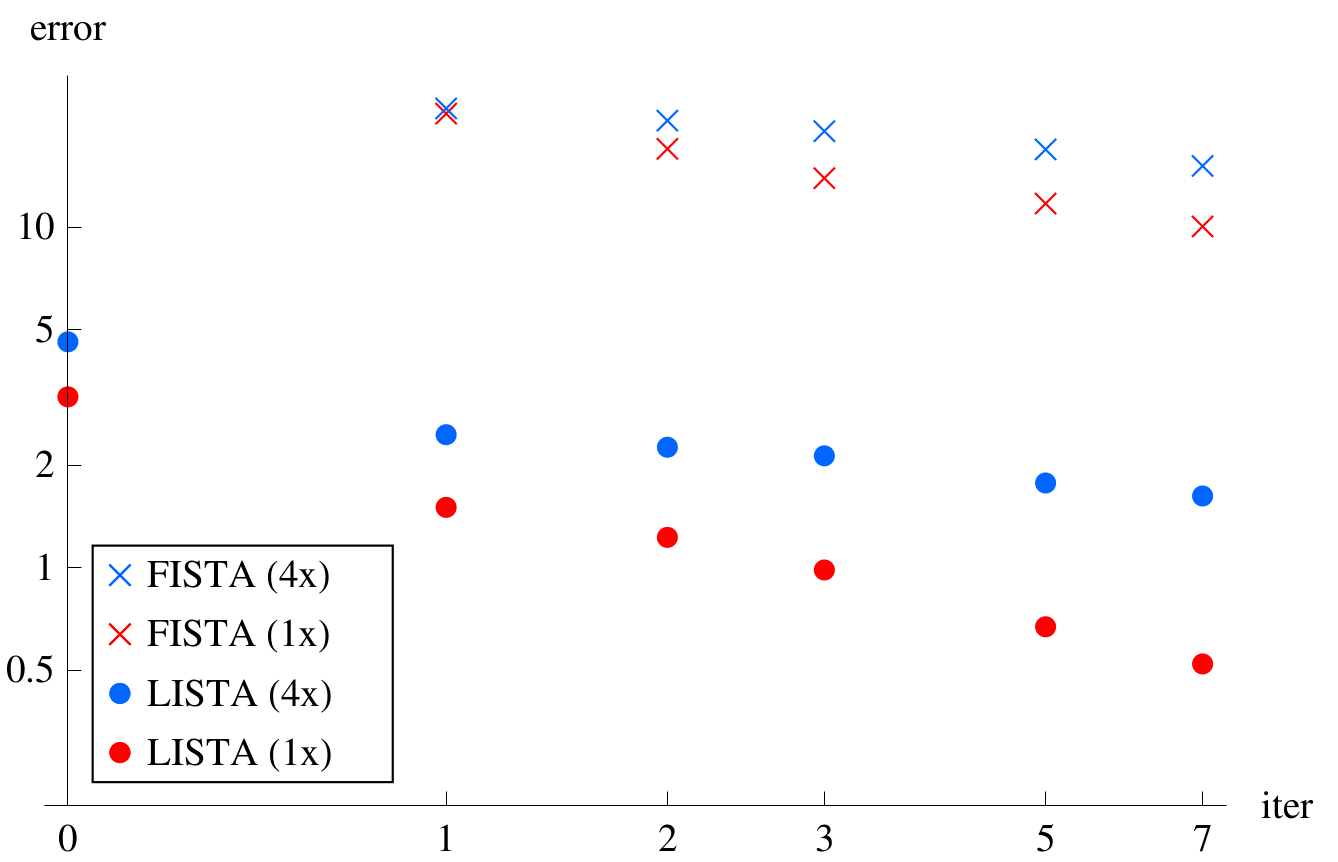
\includegraphics[width=\textwidth]{Gregor10}
		\end{subfigure}\\
		\caption*{Adapted from \cite{Gregor10}}
		\end{figure}\vskip-.5em
	}
	\only<3>{
		\vskip5em
		\textbf{Open problem: Why does it work?}\\[1em]
		\begin{itemize}\itemsep1em
			\item Can we leverage the structure of $\pmb D$?
			\item Can we get a non-asymptotic acceleration of ISTA?
			\item How to explain LISTA performance?
		\end{itemize}
		\vskip2em
		\mycite{Giryes2016, xin2016maximal}
	}
}
\end{frame}

\begin{frame}

	\twocols{
	\btitle{Notations}
	\vskip2em
	Consider the sparse coding problem with a dictionary $D$.\\[.5em]
	\[
		z^{*} = \argmin_{z} F(z) = 
				\underbrace{\| x - D z\|_2^2}_{E(z)}
				+ \lambda\| z\|_1
	\]
	\vskip1em
	We denote $B = D\tran D$ is the Gram matrix of $D$.\\[3em]
	
	\uncover<2>{\bf We introduce a novel class of algorithms -- FacNet --
				based on a sparse factorization of $B$.}
	
	}{
	\vskip3em
		Quadratic form: $Q_S(u, v) = \frac{1}{2}(u-v)\tran S (u-v) + \lambda \|u\|_1~.$\\[2em]
		
		Note that $F(z) = Q_B(z, D^\dagger x)$\\[2em]
		For $S$ is diagonal, $\argmin_u Q_S(u, v)$ can be efficiently minimized as
		the problem is separable on each coordinate:
		\[
			\argmin_{u_i}\frac{s_i}{2}(u_i - v_i)^2 + \lambda\|u_i\|
		\]
		\hskip2em $\Rightarrow$  Scaled soft thresholding
		\[
			u_i^* = \frac{\text{sign}(v_i)}{s_i}\max(0, |v_i| - \lambda)
		\]
	
	}
\end{frame}



%----------------------------------------------------------------
\subsection{Adaptive ISTA: FacNet}
%----------------------------------------------------------------


\begin{frame}[t]{Toward an adaptive procedure \mycite{Moreau2017}}

	\twoblocks{Toward an adaptive procedure}{
	\vskip1em
	Given an estimate $z^{(q)}$ of $z^*$ at iteration $q$, we can write:
	\begin{eqnarray*}
		F(z) & =& E(z) + \lambda\|z\|_1\\
		     & = & E(z^{(q)}) + \left\langle \nabla E(z^{(q)}) , z-z^{(q)} \right\rangle
						+ Q_{\makebox[.7em][c]{$B$}}(\phantom{\bf A}z, \phantom{\bf A}z^{(q)})~,\\
	\end{eqnarray*}%
	\vskip-1em
	\only<1>{\color{lightblue!70}}%
	\uncover<2->{\underline{ISTA:} ~~~~~Replace $B$ by diagonal matrix $S = \|B\|_2\pmb I_K$ \\[.5em]}
	\uncover<3->{\underline{\bf FacNet:} ~~Replace $B$ by $A\tran S A$ ~~~($S$ diagonal, $A$ unitary)}
	\only<-2>{\color{black}}\\
	\vskip-.5em
	\def\surogate{\alt<2>{F_q(z)}{\widetilde F_q(z)}}
	\begin{eqnarray*}
	\only<2->{
		\surogate{} & = & E(z^{(q)}) + \left\langle \nabla E(z^{(q)}) , z-z^{(q)} \right\rangle
						+ Q_{\color{blue!75}\pmb S\visible<3->{_q}}
							(\visible<3->{{\color{blue!75}\pmb A_q}}z, \visible<3->{{\color{blue!75}\pmb A_q}}z^{(q)})~,\\
			   \min_z \surogate{} &\Leftrightarrow& \min_z Q_{S\visible<3->{_q}}\Big(\visible<3->{A_q}z, \visible<3->{A_q}z^{(q)}
			   	- \text{\makebox[2.5em][c]{$S^{-1}\alt<2>{}{_qA_q}$}}\nabla E(z^{(q)})\Big)
	}
	\end{eqnarray*}
	\uncover<4>{
	Can we choose $A_q, S_q$ to accelerate the optimization compared to ISTA?}
	}{}{
		\centering
		\hskip2em
		\makebox[.75\textwidth][c]{
		\only<1>{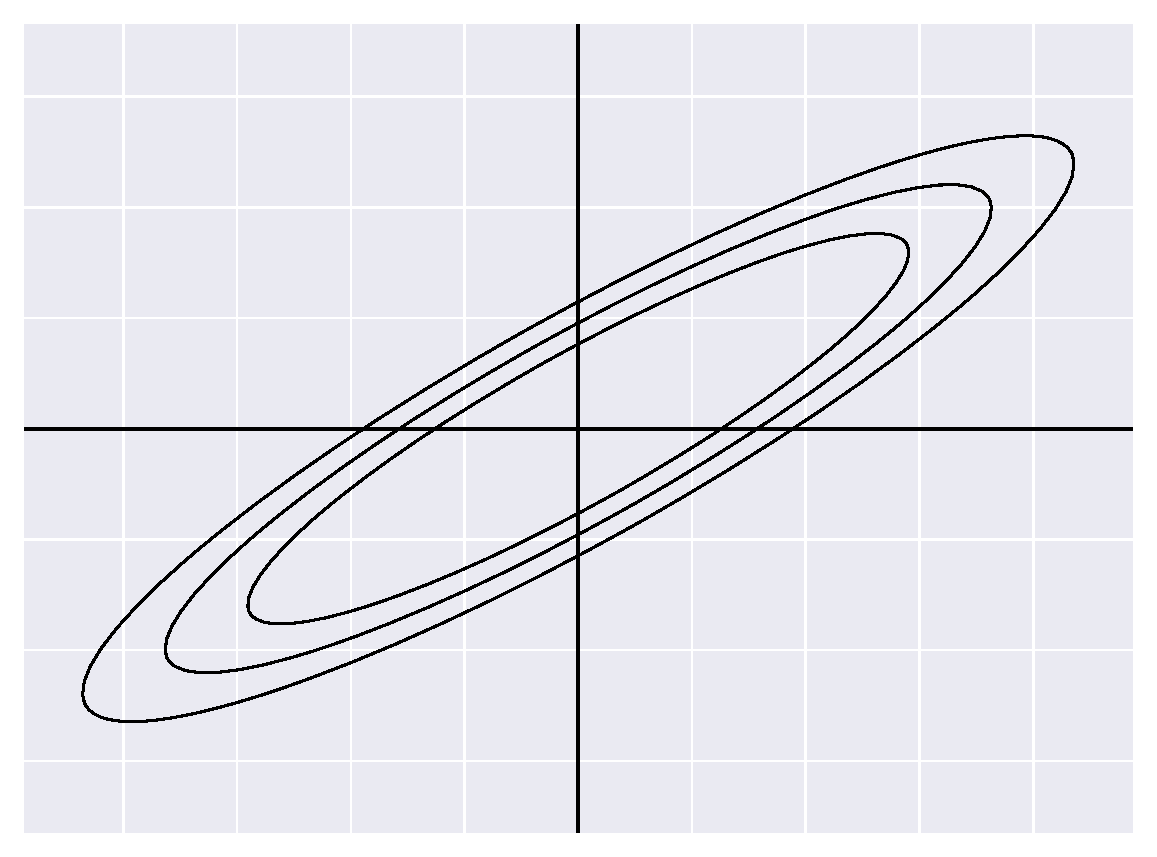
\includegraphics[height=.75\textheight]{ell1}}%
		\only<2>{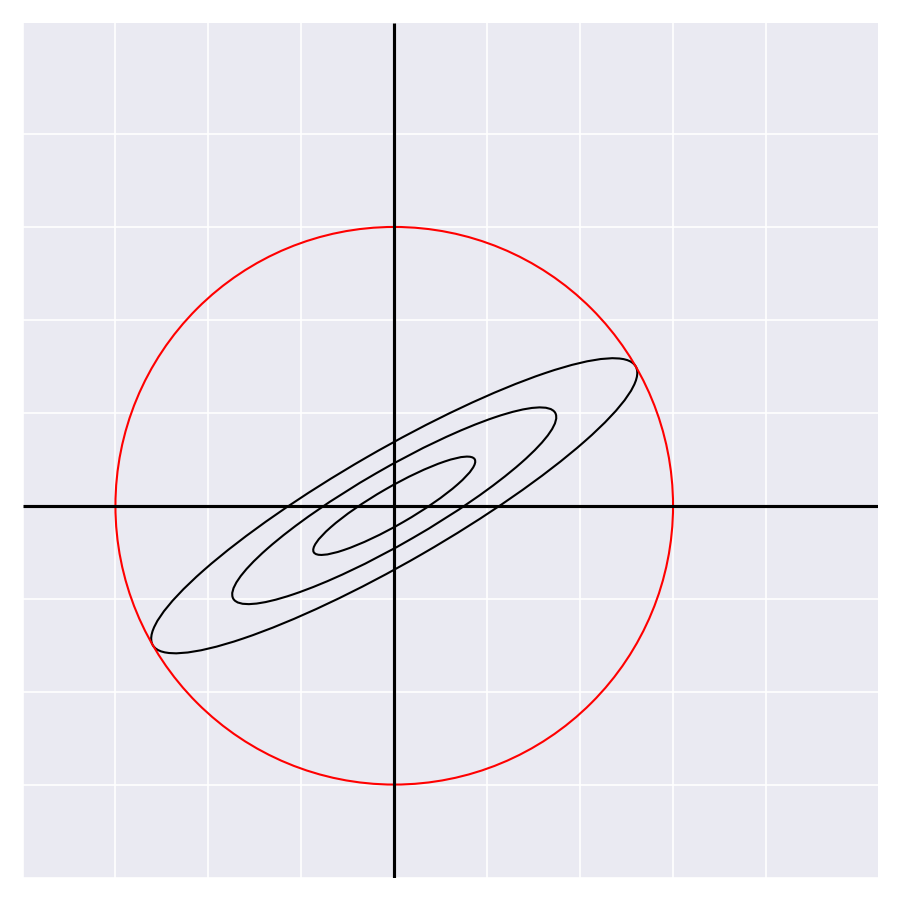
\includegraphics[height=.75\textheight]{ell2}}%
		\only<3->{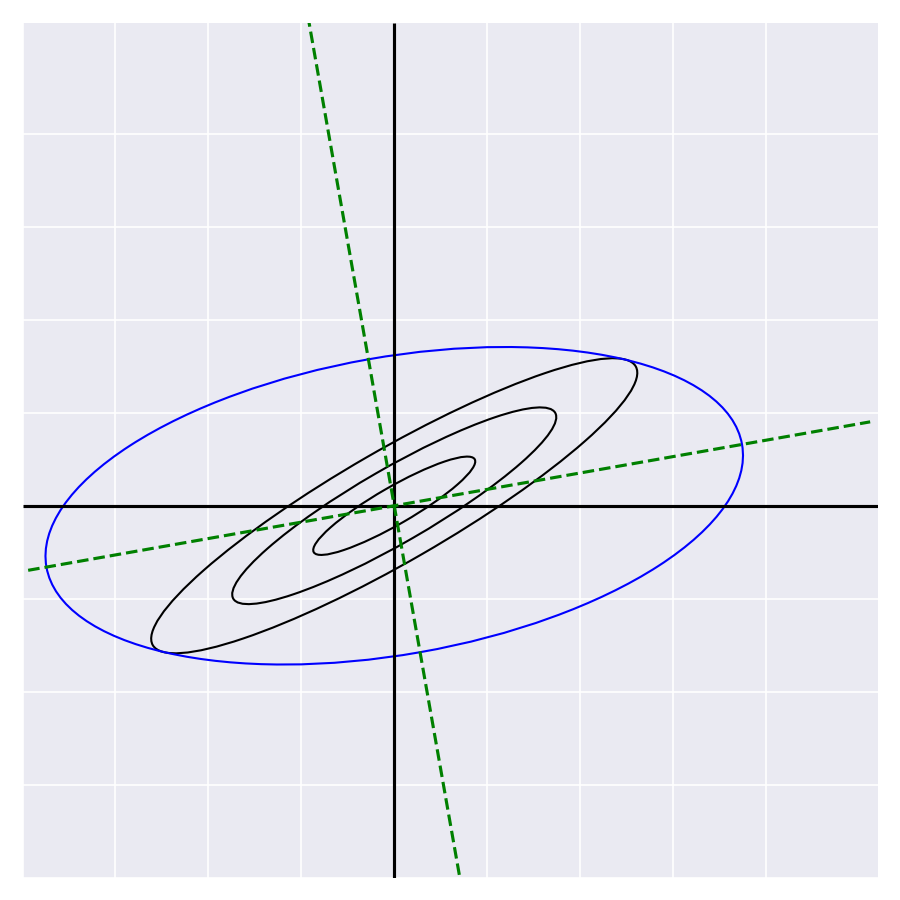
\includegraphics[height=.75\textheight]{ell3}}
		}\\
	}
\end{frame}


\begin{frame}{Toward an adaptive procedure}
	
	\twoblocks{}{

	Similar iterative procedure with steps adapted to the problem topology.\\[1em]
	\[
		\widetilde{F_q}(z) = F(z) + (z-z^{(q)})\tran R(z-z^{(q)}) + \delta_A(z)
	\]
%\textbf{Proximal resolution :}
%\[z^{(q+1)} = \argmin_z F(z) = E(z^{(q)}) + \langle B(z^{(q)}-y) , z-z^{(q)} \rangle + \frac{1}{2}\| z - z^{(q)} \|_B^2 + G(z)~ ,\]
%$\color{darkblue}\Rightarrow$ Not computationally efficient but quick minimization.\\[1.5em]


	Tradeoff between:\\[.3em]
	\begin{itemize}\itemsep1em
		\item Rotation to align the norm $\|\cdot\|_B$ and the norm $\|\cdot\|_1$~,
		\keypoint{Computation}
		\[ R = A\tran SA - B\]
		\item Deformation of the $\ell_1$-norm with the rotation $A$~.
		\keypoint{Accuracy}
		\[ \delta_A(z) = \lambda\left(\|Az\|_1-\|z\|_1\right) \]
	\end{itemize}
	}{One step improvement}{
	\begin{block}{}
		\label{bi1}
		Suppose that $R = A\tran S A - B \succ 0$ is positive definite, and define 
		\[z^{(q+1)} = \arg\min_z \widetilde{F_q}(z)~,\]
		Then
		\[
		\begin{split}
			F(z^{(q+1)}) - F(z^*) \leq \frac{1}{2}(z^{(q)} - z^*)\tran R (z^{(q)} - z^*)~~~~~\\
									+ \delta_A(z^*) - \delta_A(z^{(q+1)})~.
\end{split}
		\]
	\end{block}
	\vskip1em
	We are interested in factorization $(A, S)$ for which $\|R\|_2$ and $\delta_A$  are small.}
\end{frame}



\begin{frame}{Adaptive Iterative Soft thresholding - Convergence rate}

	\twocols{
    \begin{block}{Theoretical results}
    \vskip1em
    \begin{itemize}\itemsep1em
		\item We showed that FacNet has the same asymptotic convergence rate as ISTA
		in $\mathcal O(\tfrac{1}{q})$.
		\item The constant factors are different and can be improved.
		If the factorization $(A_q, S_q)$ at iteration $q$  verifies
			\[
				\|R_q\|_2 + 2 \frac{L_{A_q}(z^{(q+1)})}{\|z^*-z^{(q)}\|_2} \le \frac{\|B\|_2}{2}
			\]
			and $A_p = \pmb I_K, S_p = \|B\|_2\pmb I_K$ for $p > q$, then the procedure has
			improved convergence rate compared to ISTA.\\[1em]
			{{\usebeamercolor[fg]{block title}$\Rightarrow$}} There is a phase transition when
			 $\|z^{(q)} - z^*\|_2 \to 0$
	\end{itemize}
    \end{block}
    }{
    \vskip2.7em
    \begin{itemize}\itemsep1em
    	\item We consider the \textbf{generic dictionaries}, uniformly sampled
    	from $\mathcal S^{p-1}$.
		\item We derive \textbf{sufficient conditions} on the problem setting for
		the existence of a factorization $(A_q, S_q)$ of $B$ which improves
		\textbf{the performance of one step} of FacNet compared to one step of ISTA,
		\textbf{in expectation over the \emph{generic dictionaries}}.
		\[\begin{split}
			\lambda\E[z]{\|z^{(q+1)}\|_1+\|z^*\|_1}\le\hskip6em\\
				\sqrt{\frac{K(K-1)}{p}} \E[z]{\|z^{(q)}-z^*\|_2^2}
		\end{split}\]
	\end{itemize}
	}
\end{frame}



%---------------------------------------------------------
\subsection{Understanding LISTA}
%---------------------------------------------------------

\begin{frame}
\twoblocks{Learned ISTA \mycite{Gregor10}}{
	\vskip1em
		\centering
		\inputTikZ{.8}{ista_tikz.tex}\\
		\inputTikZ{.8}{lista_tikz.tex}\\
		Network architecture for ISTA/LISTA. LISTA is the unfolded version
				 of the RNN of ISTA, trainable with back-propagation.
	\vskip1em
	With $W_e = \frac{D\tran}{\|B\|_2} $ and $W_g = I - \frac{B}{\|B\|_2}$, this network computes exactly 2 iterations of ISTA.
}{\only<2>{FacNet}}{\only<2>{
	\vskip2em
	Specialization of LISTA
		\[
			z^{(q+1)} = A\tran \prox_{S}( Az^{(q)} - S^{-1}A B(z^{(q)} - y))~,
		\]
		with $A$ unitary and $S$ diagonal.\\
	Same architecture with more constraints on the parameter space:
	\begin{equation*}
	\begin{cases}
		W_e & = S^{-1}A D\tran\\
		W_g & =  A\tran - S^{-1}A BA\tran
	\end{cases}
	\end{equation*}
	\vskip2em
	\hskip3em $\Rightarrow$ LISTA can be at least as good as this model.
}}
\end{frame}



\begin{frame}{Artificial simulation}
\twocols{
	\begin{block}{Generic Dictionary}
	\vskip1em
	\begin{itemize}\itemsep1em
		\item Generic dictionary uniformly sample in unit ball,
		\[
			D \sim \mathcal S^{p-1}~,
		\]
		\item Sparse code generated with Bernouilli-Gaussian model, \emph{s.t.}
		\[z_k = b_ka_k, \hskip2em b_k \sim \mathcal B(\rho) \text{ and } a \sim \mathcal N(0, \sigma \pmb I_K)\]
	\end{itemize}
	\vskip1em 
	\emph{Fixed: } $K = 100$, $P = 64$, $\sigma = 10$ and $\lambda = 0.01$
	\end{block}
	}{
		\centering
		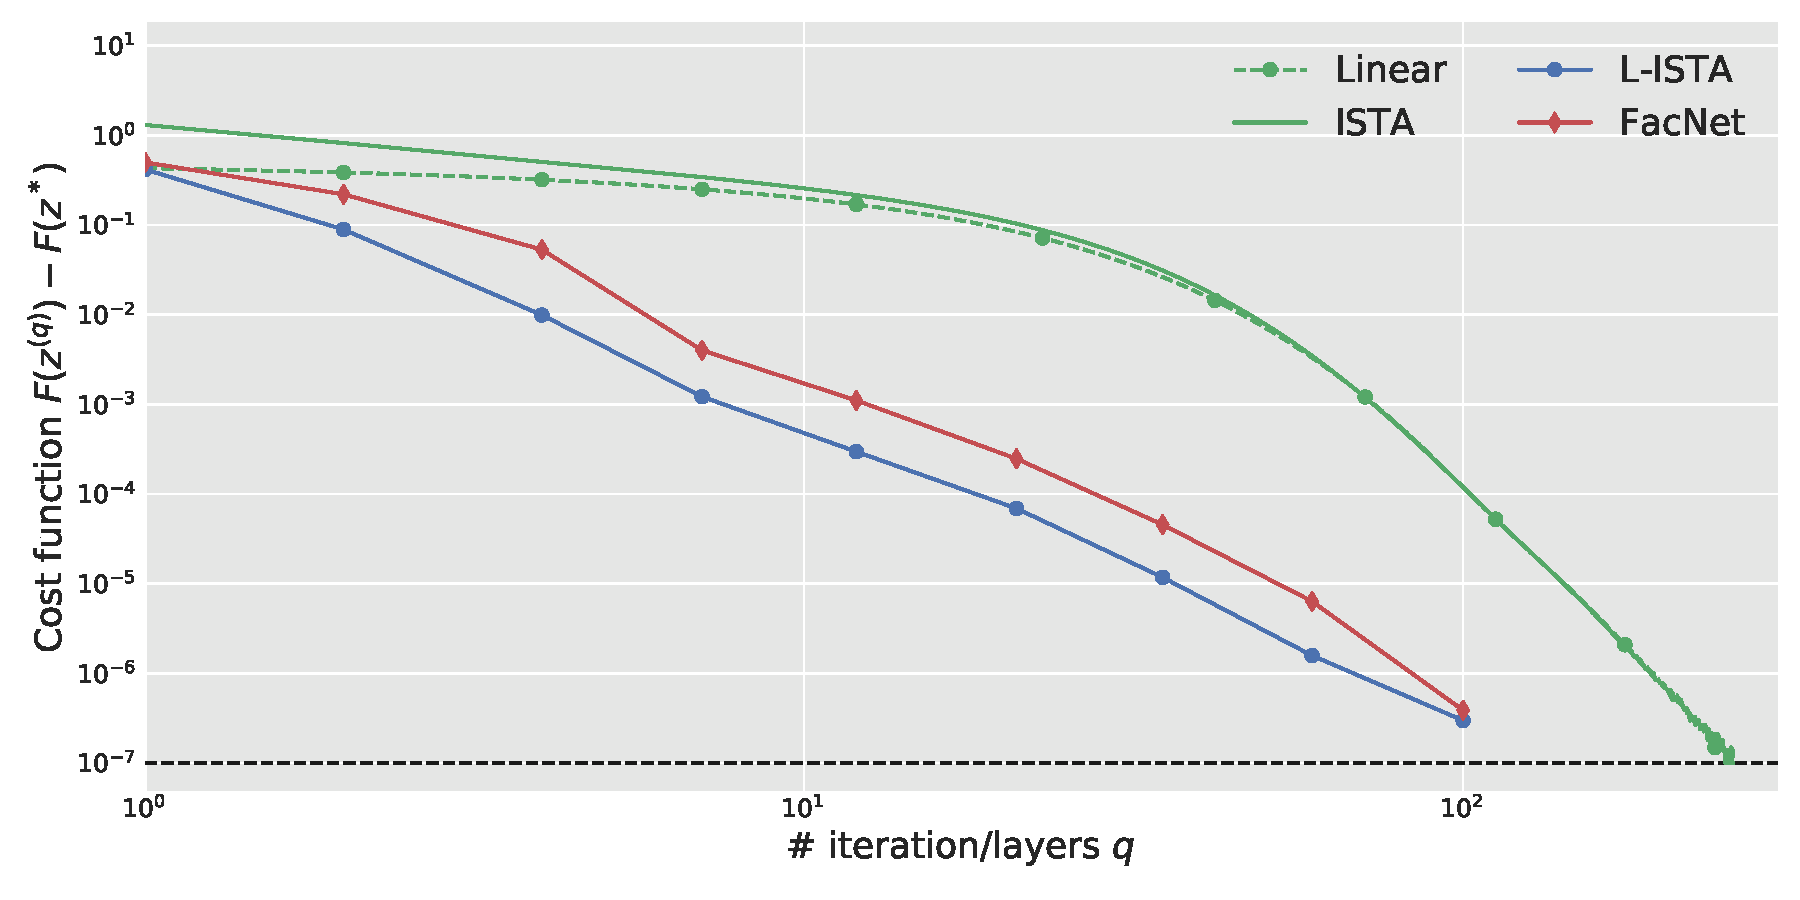
\includegraphics[width=\textwidth]{curve_sparse005_seaborn_min}\\
		$\rho = {}^1/_{20}$.\\[1em]

%	\only<2>{
%		\includegraphics[width=\textwidth]{curve_sparse02_seaborn_min}\\
%		$\rho = {}^1/_{4}$.\\[1em]
%	}
		Evolution of the cost function $F(z^{(q)}) - F(z^*)$ with the number
	   	of layers/iterations $q$ with a denser model
	}
\end{frame}




\begin{frame}{Adversarial dictionary}

	\twocols{
		\begin{block}{Adversarial dictionary}
		\vskip2em
		The dictionary is constructed such that it eigen-vectors are sampled from the
		Fourier basis, with
		\[
			D_{k, j} = e^{-2i\pi k \zeta_j}
		\]
		for a random subset of frequencies
		\[
			\left \{ \zeta_i \right \}_{0\le i \le p} \sim \mathcal U \left\{\frac{m}{K}; 0 \le m \le \frac{K}{2}\right\}
		\]
		Diagonalizing $B$ implies large deformation of the $\ell_1$-norm. 
\end{block}
		%\includegraphics[width=\textwidth]{dictionary}
	}{%
	%\vskip4em
\centering
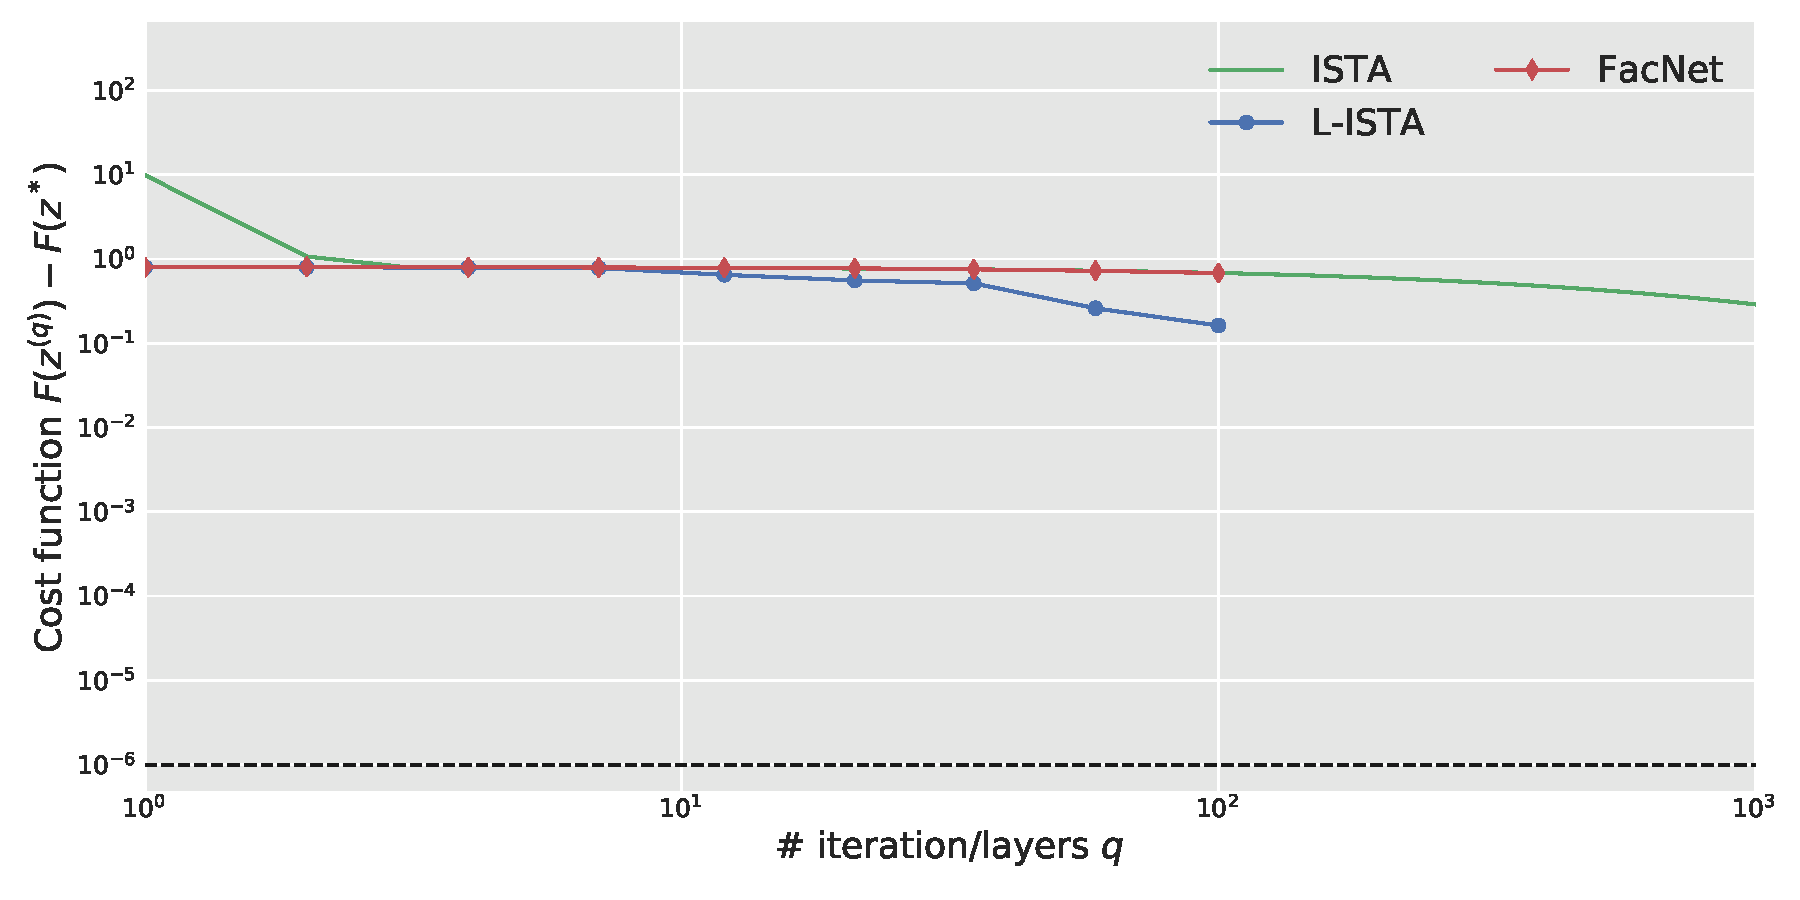
\includegraphics[width=\textwidth]{curve_adverse_seaborn_min}\\
    Evolution of the cost function $F(z^{(q)}) - F(z^*)$ with the number of layers/iterations $q$ 
    with an adversarial dictionary.
    }
\end{frame}


\begin{frame}{Contribution}

	\twoblocks{Contributions}{
	\vskip1em
	\begin{itemize}\itemsep1.5em
		\item \underline{Theoretical analysis:} Non asymptotic acceleration of ISTA is possible
		based on the structure of $\pmb D$,
		\item \underline{FacNet Algorithm:} Sufficient analysis to explain LISTA acceleration,
		\item \underline{Adversarial Example:} Empirically showed the structure of $D$ is necessary
		for LISTA. 
	\end{itemize}

    }{Future work}{
	\vskip1em
	\begin{itemize}\itemsep1.5em
	    \item Direct factorization: Improve the factorization formulation
	    for direct optimization,
	    \item Performance quantification: Second order analysis for generic dictionary,
	    \item Sparse PCA: Link the sparse eigenvectors properties to our factorization.
    \end{itemize}}
	
\end{frame}






%===========================================================================
\section{Conclusion}
%===========================================================================

\begin{frame}{Conclusion}
\twocols{
	\begin{block}{A diverse work}
		\begin{itemize}
			\item Technical contributions:\\
			$\rightarrow $  Theoretical study of LISTA; DICOD
			\item Exploratory contributions:\\
			$\rightarrow $ Link SSA to CSC; Post-training
			\item Collaboration with Medical doctors for clinical research publications,
			\item Contribution to open source software with the python library \code{loky}.
		\end{itemize}
	\end{block}

	\begin{block}{A collaborative work}
		\begin{itemize}
			\item Co-authors: L. Oudre, N. Vayatis, J. Audiffren,\\
							  R. Barrois, J. Bruna.
			\item Medical doctors: S. Buffat, D. Ricard, M. Robert, P-P. Vidal, C. de Waele, A. Yelnik.
			\item Open-source: O. Grisel.
		\end{itemize}
	\end{block}
}{
	\begin{block}{Publications and preprints}
		\scriptsize\vskip.5em
		\bibentry{Moreau2015a}\\[.5em]
		\bibentry{Oudre2015}\\[.5em]
		\bibentry{Moreau2015}\\[.5em]
		\bibentry{Moreau2016}\\[.5em]
		\bibentry{Moreau2017}\\[.5em]
		\bibentry{Moreau2017a}\\[.5em]
		\bibentry{Barrois2015}\\[.5em]
		\bibentry{Barrois2016}\\[.5em]
		\bibentry{Robert2015}\\[.5em]
    \end{block}
  }
\end{frame}

\begin{frame}[noframenumbering,plain]
  \begin{center}
    \Huge
    Thanks!    
  \end{center}
\end{frame}

%===========================================================================
% AUXILIARY SLIDES
%===========================================================================



%===========================================================================
\appendix
\section{Auxiliary Slides}
%===========================================================================


%===========================================================================
\subsection{Physiological Signals}
%===========================================================================


\begin{frame}

	\twocols{
		\btitle{Experiment}
		\vskip2em
		Create a dictionary with 25 Gaussian patterns ($W=90$)
		\[
			\pmb D^{(0)}_k \sim \mathcal N(0, I_{90})
		\]
		\vskip1em
		Use the Convolutional Dictionary Learning with\\
		DICOD to learn a dictionary $\pmb D$ on a set of $50$\\
		recording of healthy subjects walking.
		\vskip2em
		\btitle{Challenges}
		\vskip.5em
		\begin{itemize}\itemsep.5em
			\item Alignment of the patterns,
			\item Detect steps of different amplitude,
			\item Handle multivariate signals.
		\end{itemize}
	
	}{
		\centering
		\mbox{\hskip-2.1em
		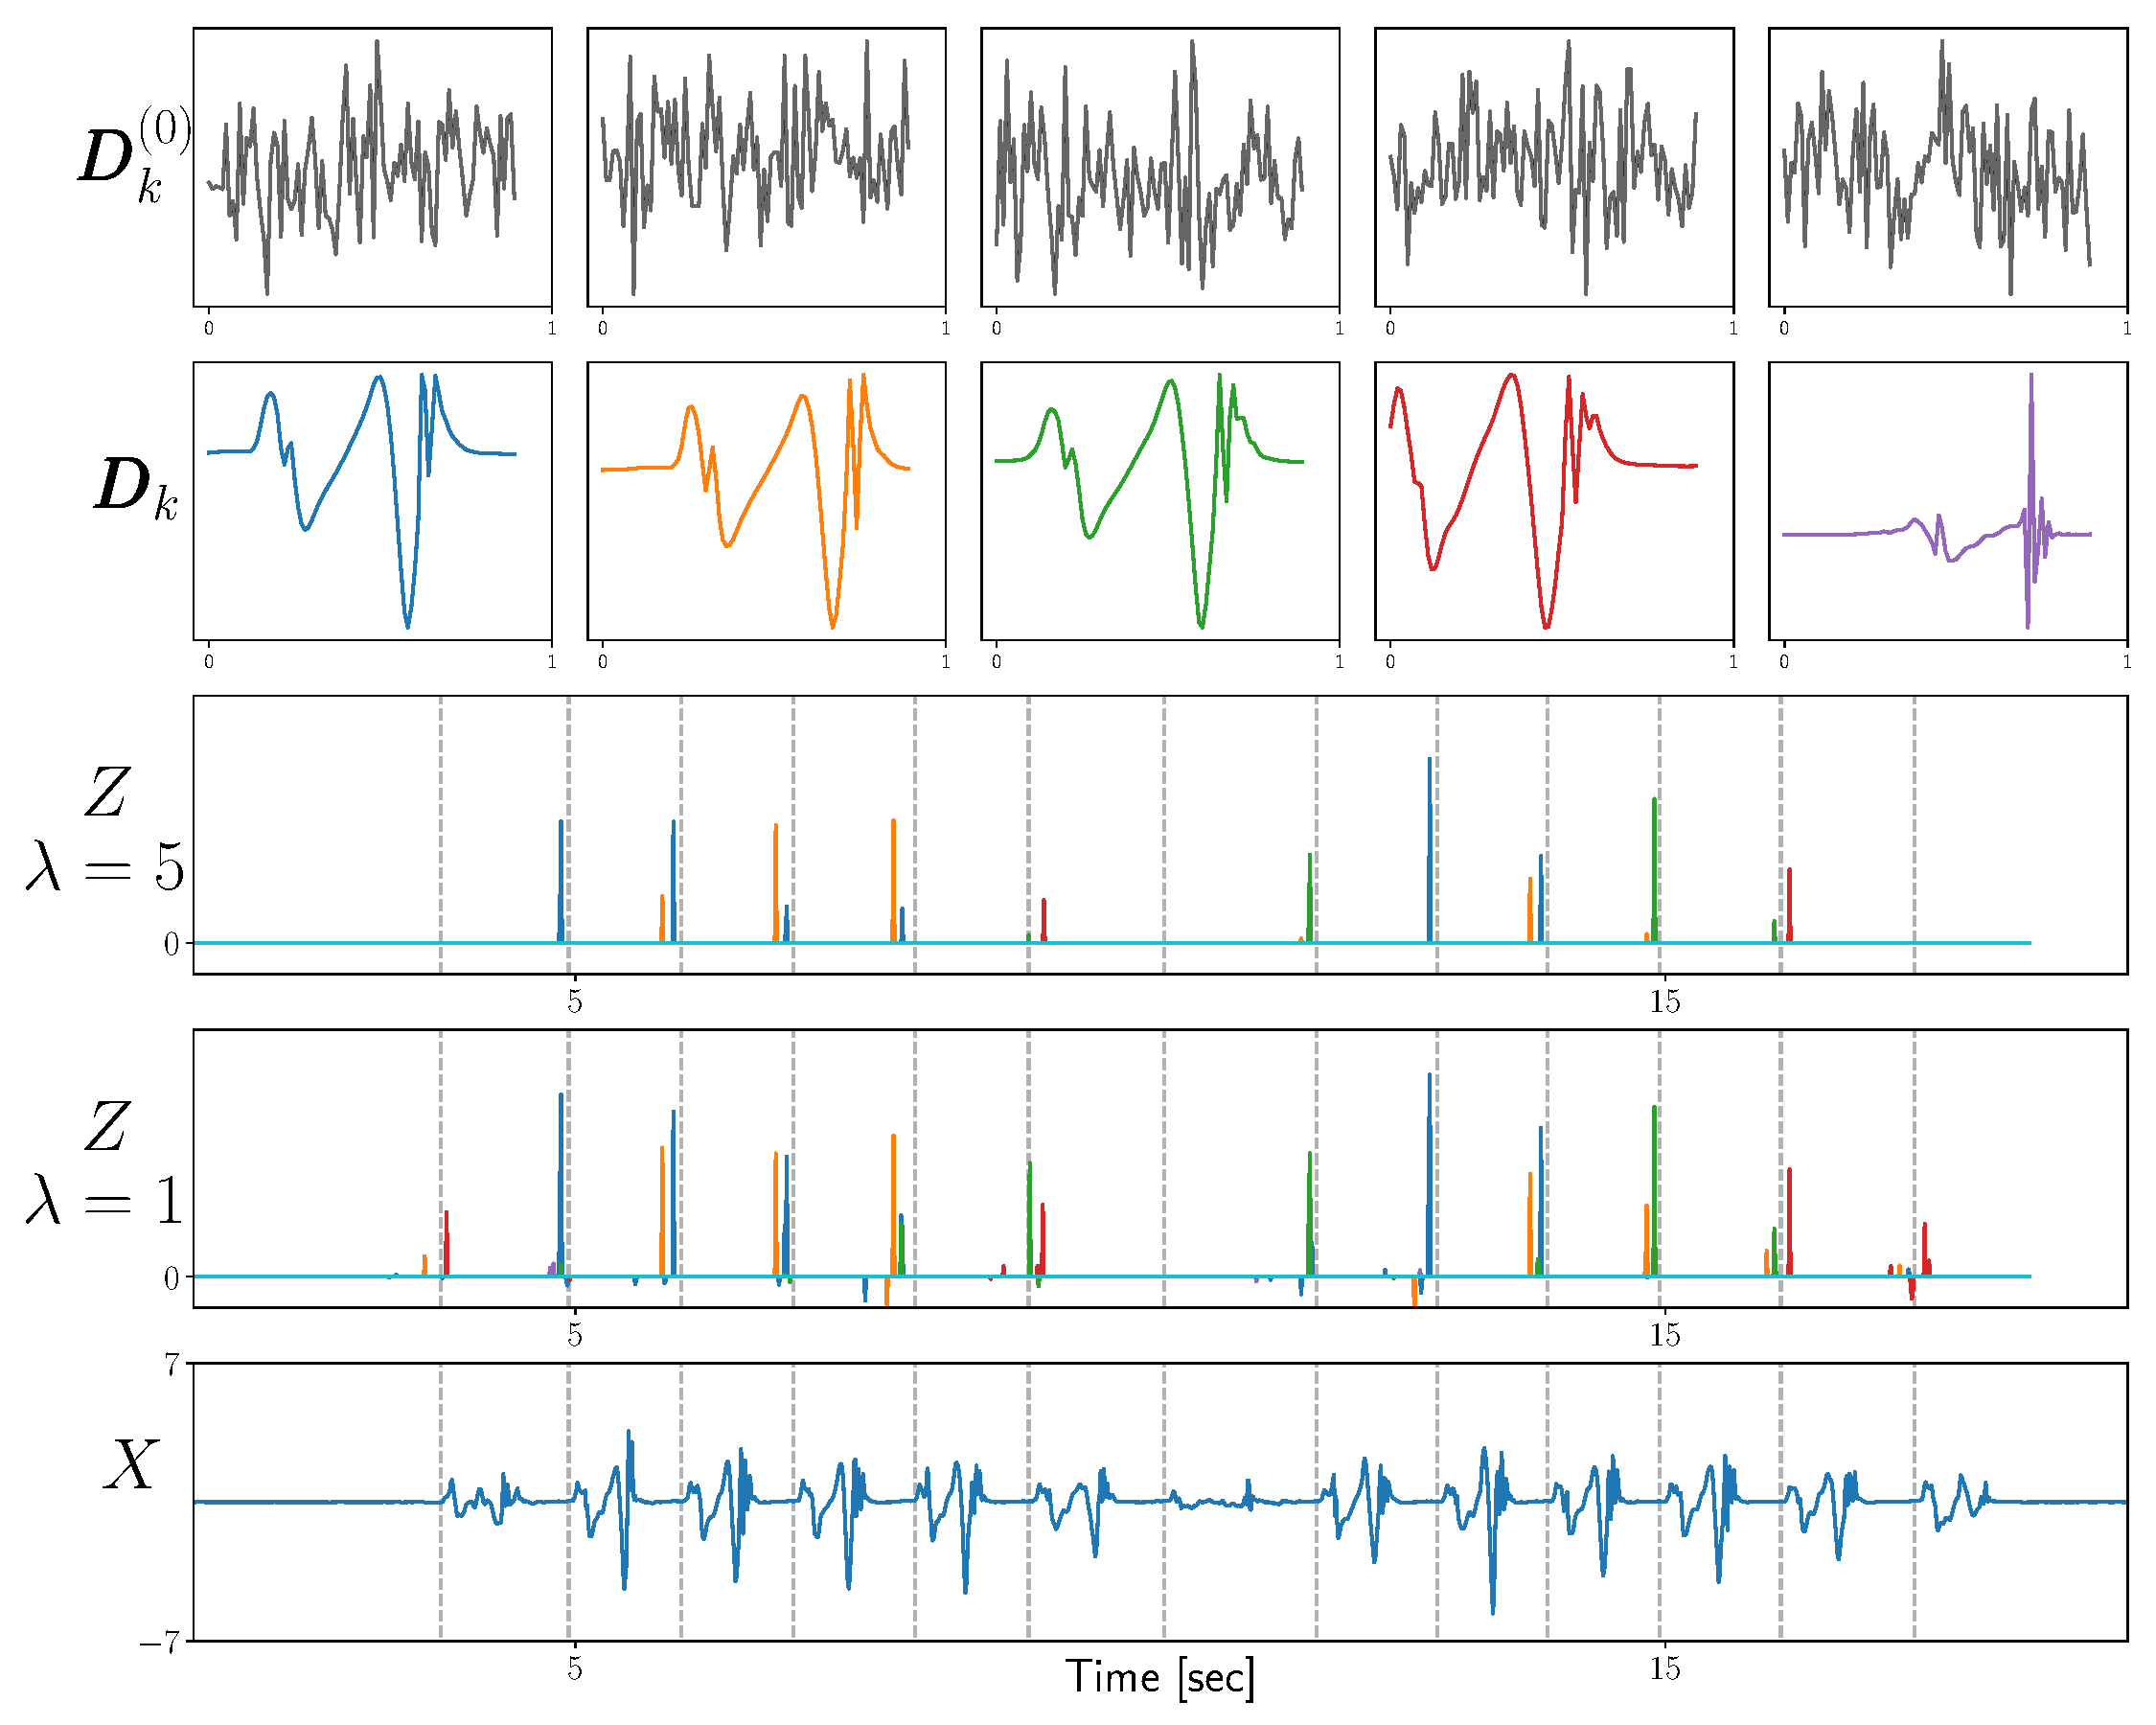
\includegraphics[width=1.1\textwidth]{csc_random_defense}}\\
	}

\end{frame}
\begin{frame}

	\twocols{
		\btitle{Experiment}
		\vskip2em
		Create a dictionary with 25 Gaussian patterns ($W=90$)
		\[
			\pmb D^{(0)}_k \sim \mathcal N(0, I_{90})
		\]
		\vskip1em
		Use the Convolutional Dictionary Learning with\\
		DICOD to learn a dictionary $\pmb D$ on a set of $50$\\
		recording of healthy subjects walking.
		\vskip2em
		\btitle{Challenges}
		\vskip.5em
		\begin{itemize}\itemsep.5em
			\item Alignment of the patterns,
			\item Detect steps of different amplitude,
			\item Handle multivariate signals.
		\end{itemize}
	
	}{
		\centering
		\mbox{\hskip-2.1em
		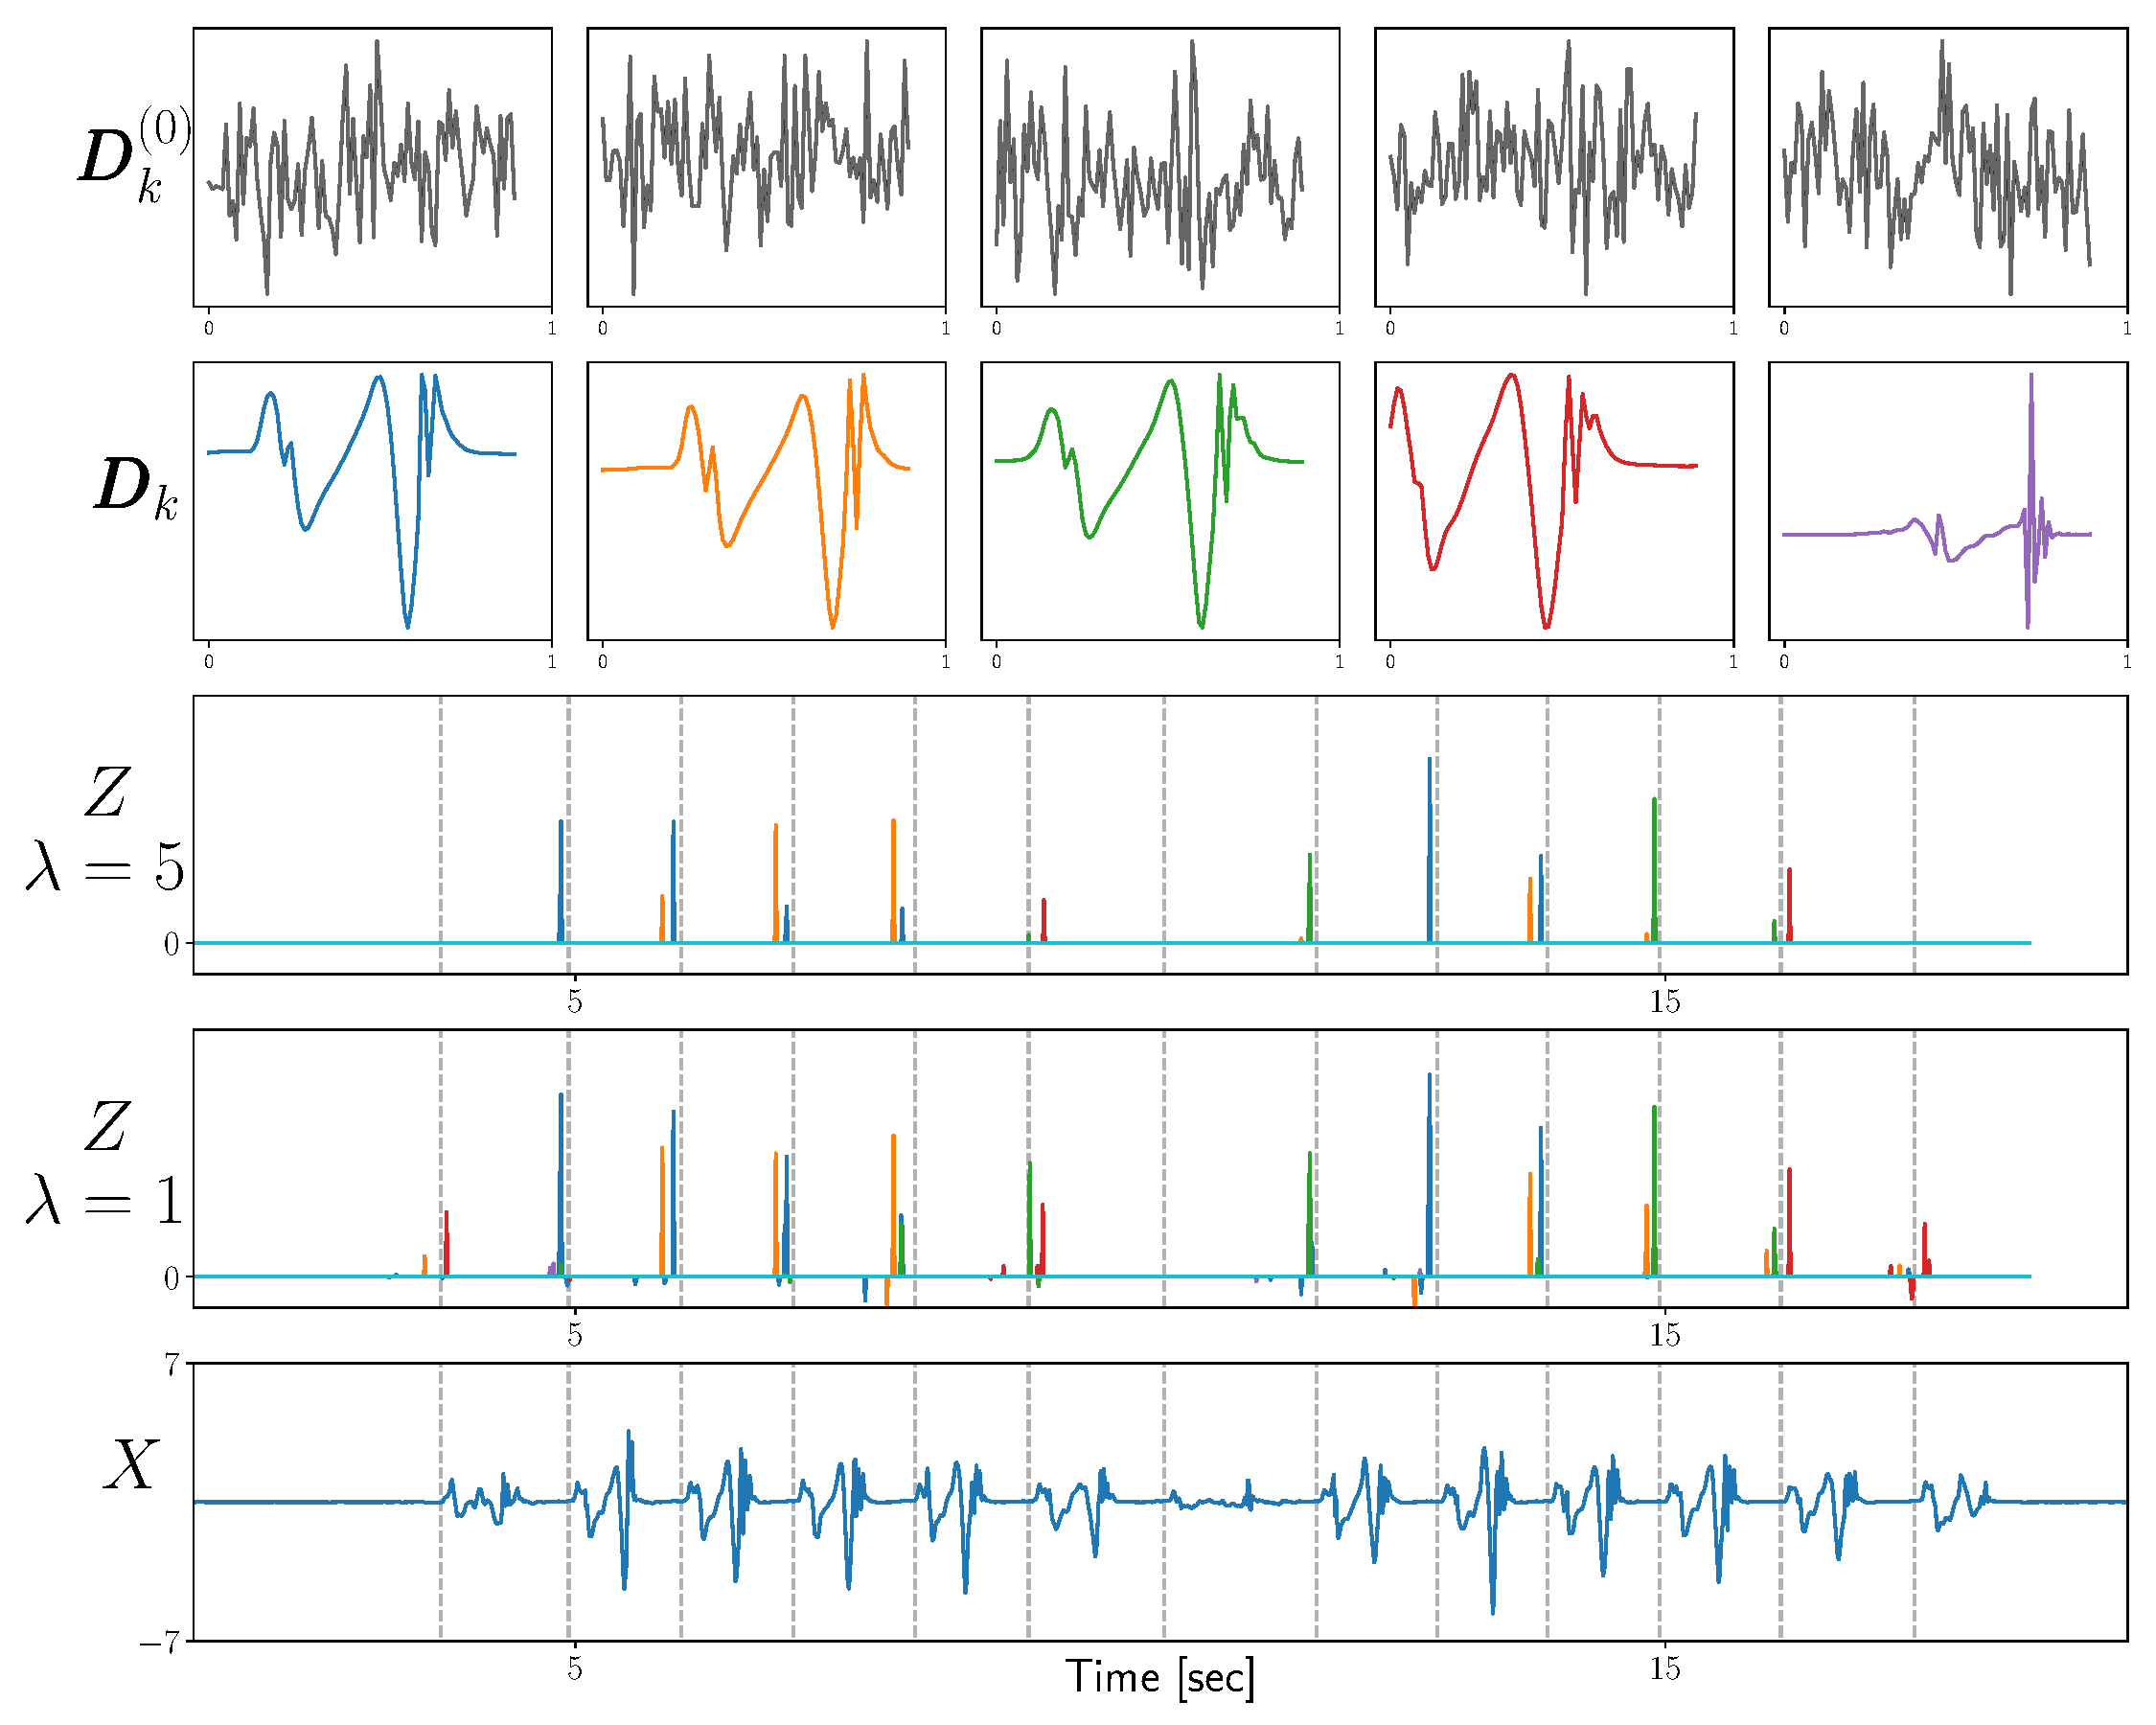
\includegraphics[width=1.1\textwidth]{csc_random_defense}}\\
	}

\end{frame}



\begin{frame}
\twocols{


}{
	\centering
	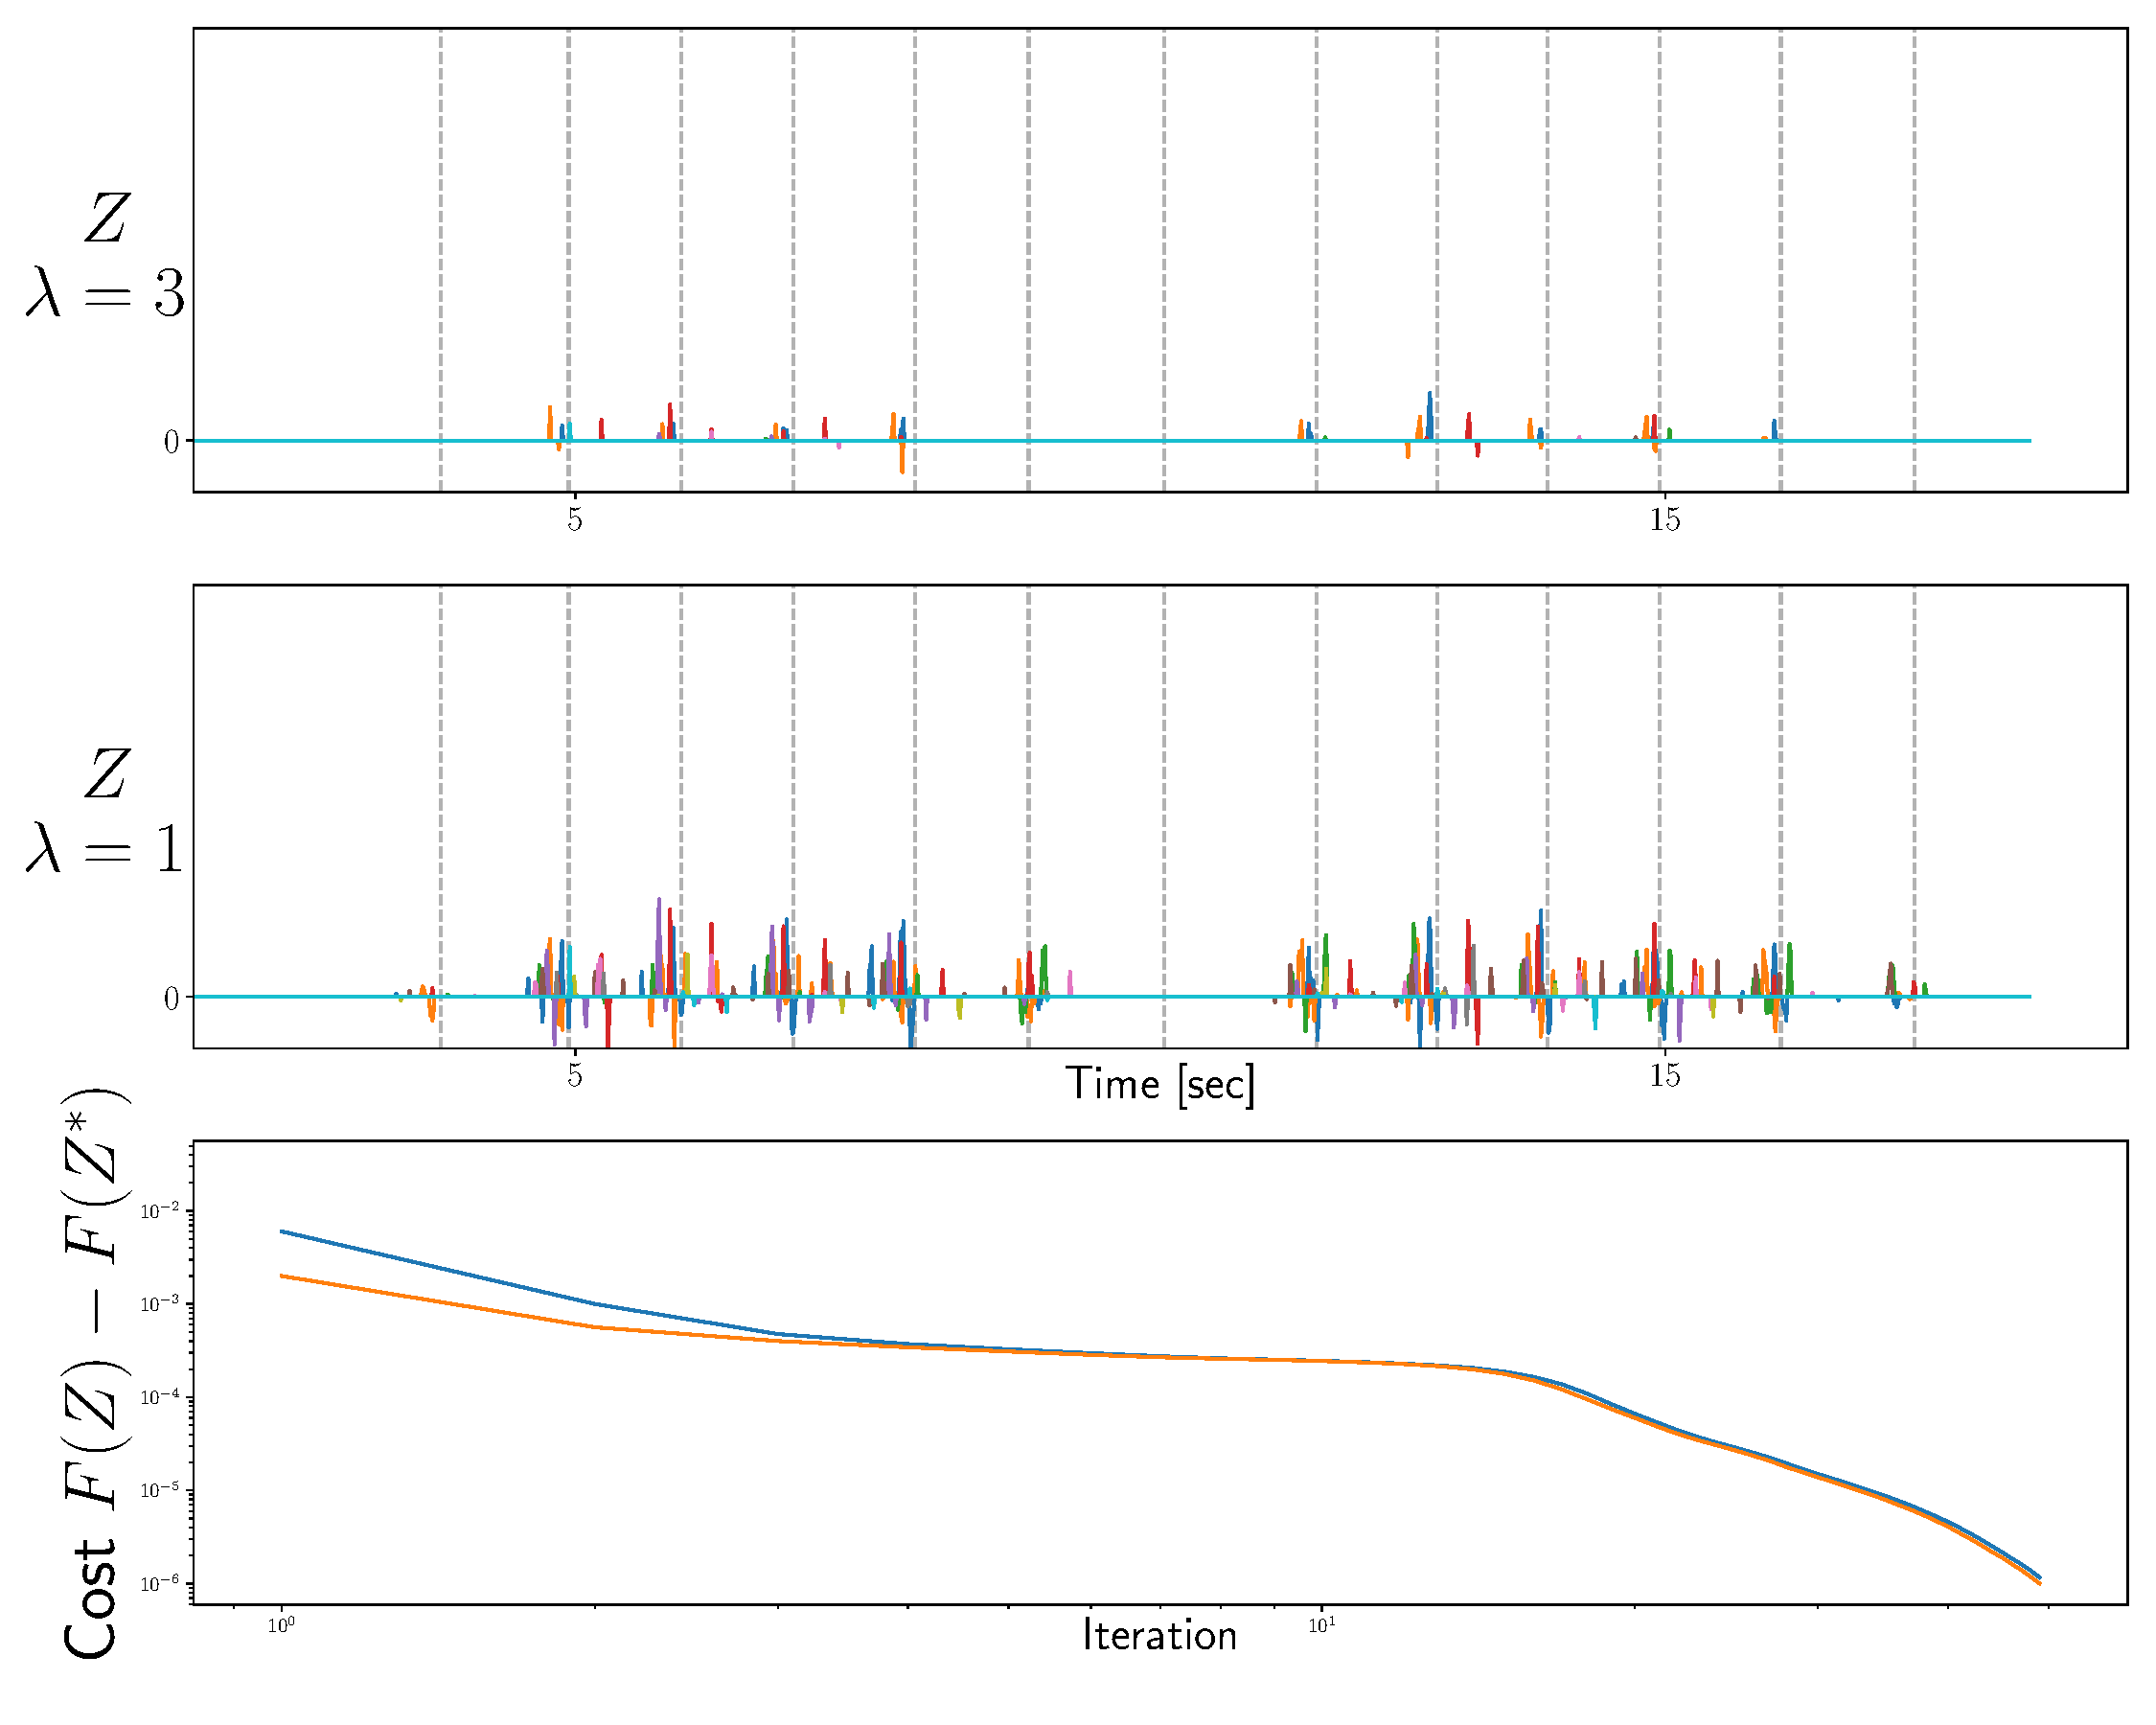
\includegraphics[width=\textwidth]{csc_random_annex}
}
	
\end{frame}

%===========================================================================
\subsection{FacNet}
%===========================================================================


\begin{frame}{Related works}

\twoblocks{}{
\begin{itemize}\itemsep2em
	\item \cite{Giryes2016}: Propose the inexact projected gradient descent and conjecture that LISTA accelerate the LASSO resolution by learning the sparsity pattern of the input distribution.
	\item \cite{xin2016maximal}: Study the Hard-thresholding Algorithm and its
	capacity to recover the support of a sparse vector.\\
	The paper relax the RIP conditions for the dictionary.
\end{itemize}
}{}{}
\end{frame}


\begin{frame}
	
	\twoblocks{Generic Dictionaries}{
	\vskip2em
	A dictionary $D \in \Rset^{p\times K}$ is a generic dictionary when its columns
	$D_i$ are drawn uniformly over the $\ell_2$ unit sphere $\mathcal S^{p-1}$.

	}{Theorem (Generic Acceleration)}{
	\vskip1em
	In \textbf{expectation over the generic dictionary} $D$, the factorization algorithm using a
		diagonally dominant matrix $A\subset\mathcal E_\delta$, has better performance for
		iteration $q+1$ than the normal ISTA iteration -- which uses the identity -- when
		\[
			\lambda\E[z]{\|z^{(q+1)}\|_1+\|z^*\|_1}
				\le \sqrt{\frac{K(K-1)}{p}} \underbrace{\E[z]{\|z^{(q)}-z^*\|_2^2}
				}_{\substack{\text{expected resolution}\\\text{at iteration $q$ }}}
		\]

	\vskip2em
	FacNet can improve the performances compared to ISTA when this is verified.}
\end{frame}



\begin{frame}
\twoblocks{L-FISTA}{
	\centering
	\vskip4em
	\inputTikZ{.65}{lifsta_tikz}
	\vskip2em
	Network architecture for L-FISTA.
}{}{
	\centering
	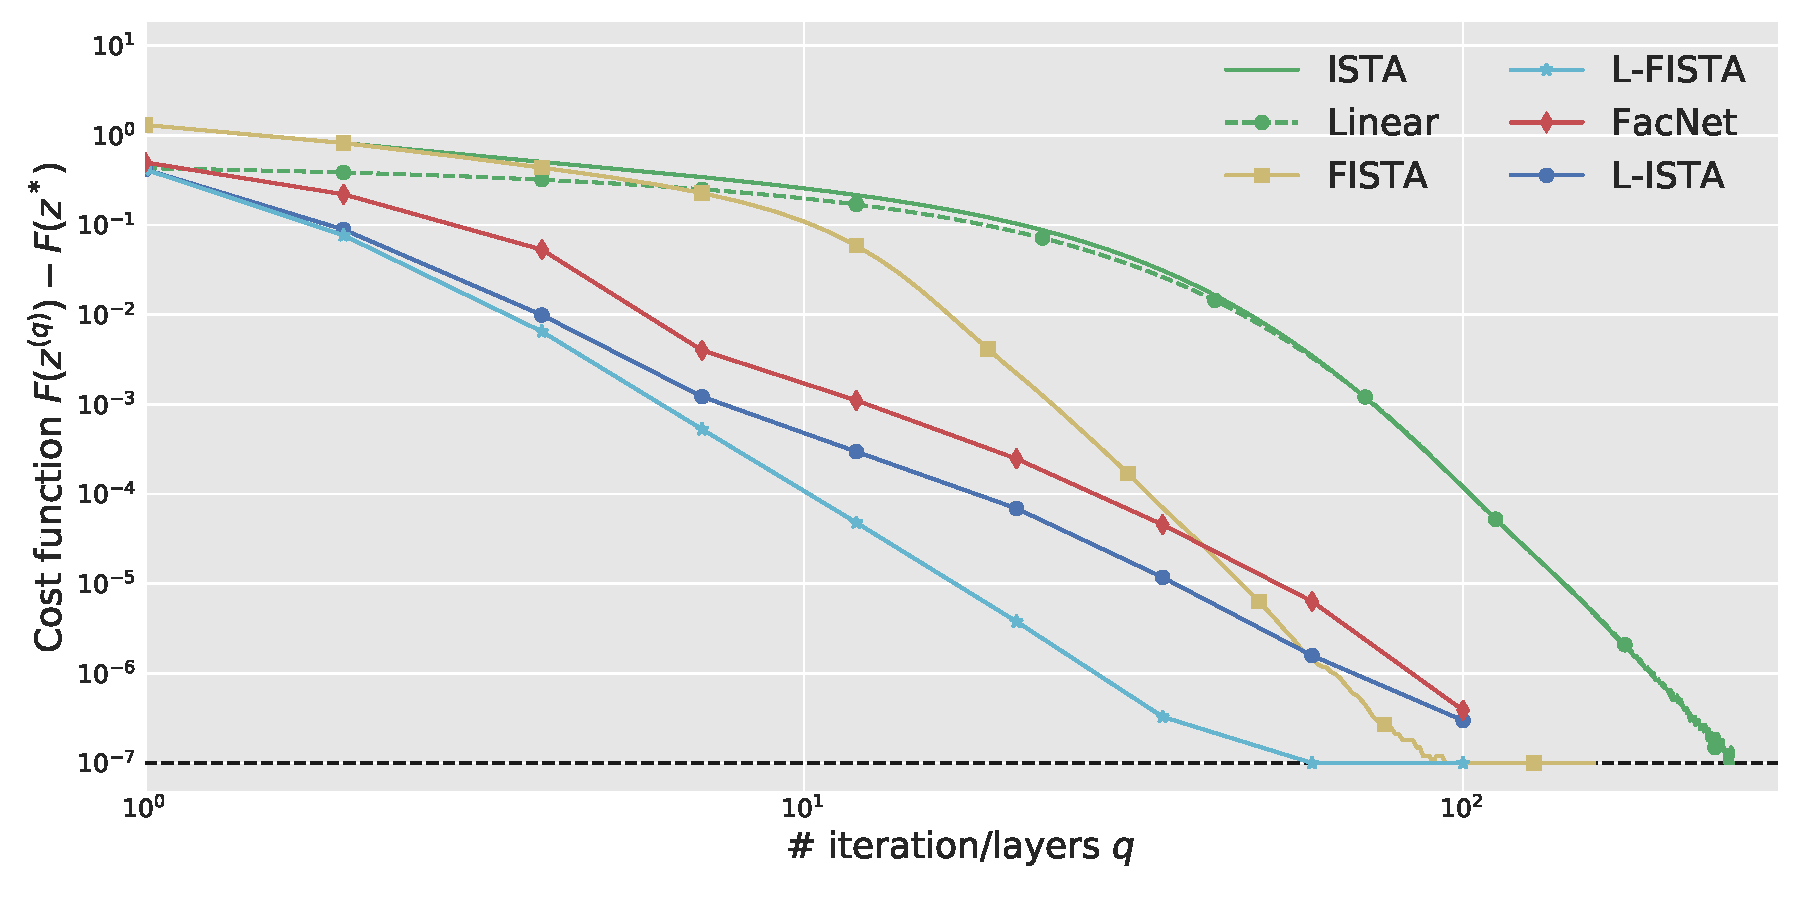
\includegraphics[width=\textwidth]{curve_sparse005_seaborn}
    Evolution of the cost function $F(z^{(q)}) - F(z^*)$ with the number
   	of layers/iterations $q$ with a denser model
}
	
\end{frame}
\begin{frame}

	\twocols{
		\centering
		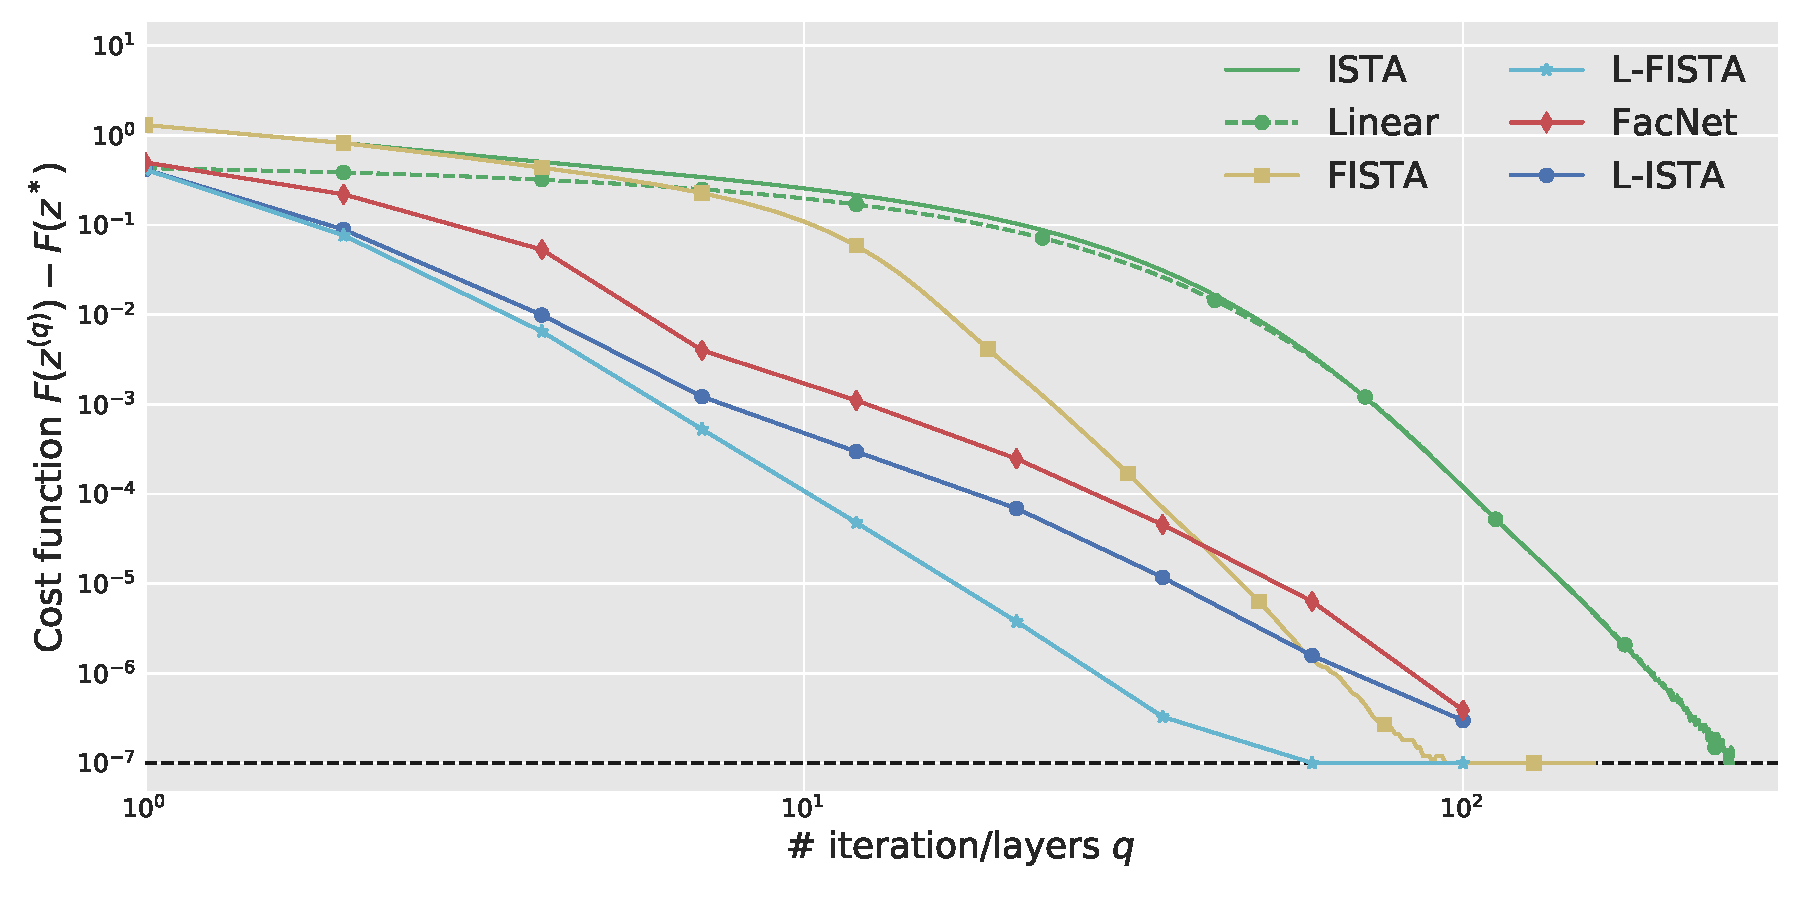
\includegraphics[width=\textwidth]{curve_sparse005_seaborn}\\
		$\rho = {}^1/_{20}$.\\[1em]

		Evolution of the cost function $F(z^{(q)}) - F(z^*)$ with the number
	   	of layers/iterations $q$ with a denser model

	}{
		\centering
		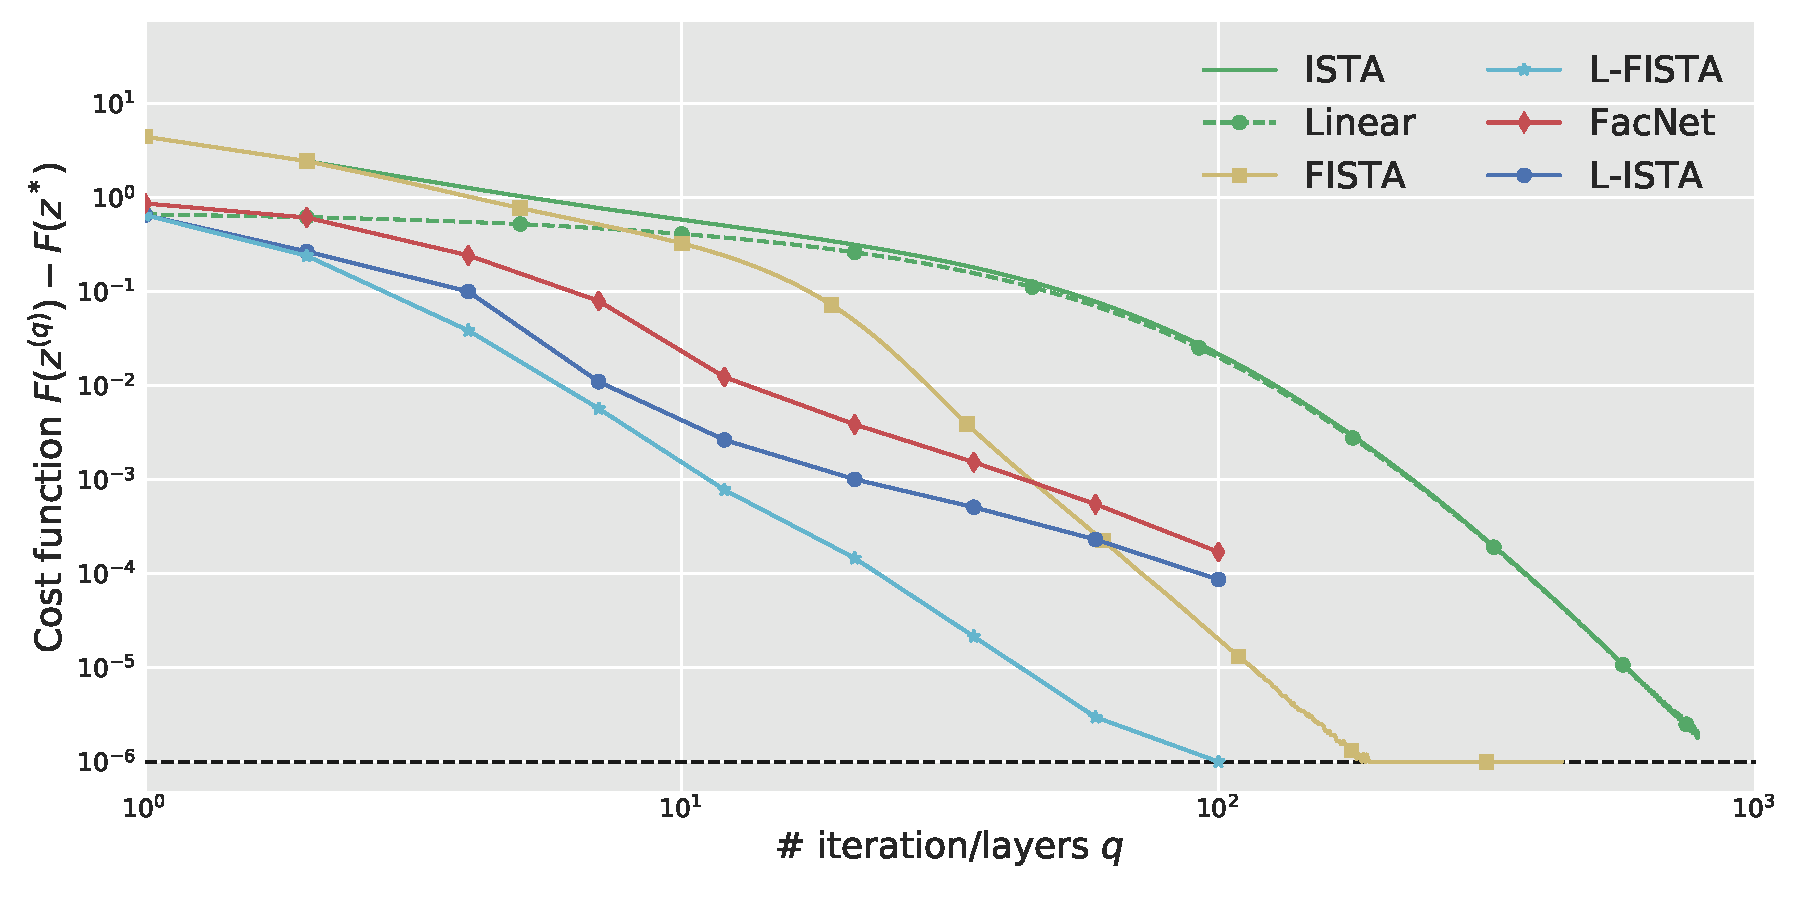
\includegraphics[width=\textwidth]{curve_sparse02_seaborn}\\
		$\rho = {}^1/_{4}$.\\[1em]
		Evolution of the cost function $F(z^{(q)}) - F(z^*)$ with the number
	   	of layers/iterations $q$ with a denser model
	}
\end{frame}


\begin{frame}{PASCAL 08}
\twocols{
	\btitle{PASCAL 08}
	\vskip1em
	Sparse coding for the PASCAL 08 datasets over the Haar wavelets family.\\[1em]
	\emph{Patch size:} 8x8;~~~$K = 267$;~~~  \emph{train/test:} 500/100\\[1em]
	\centering
	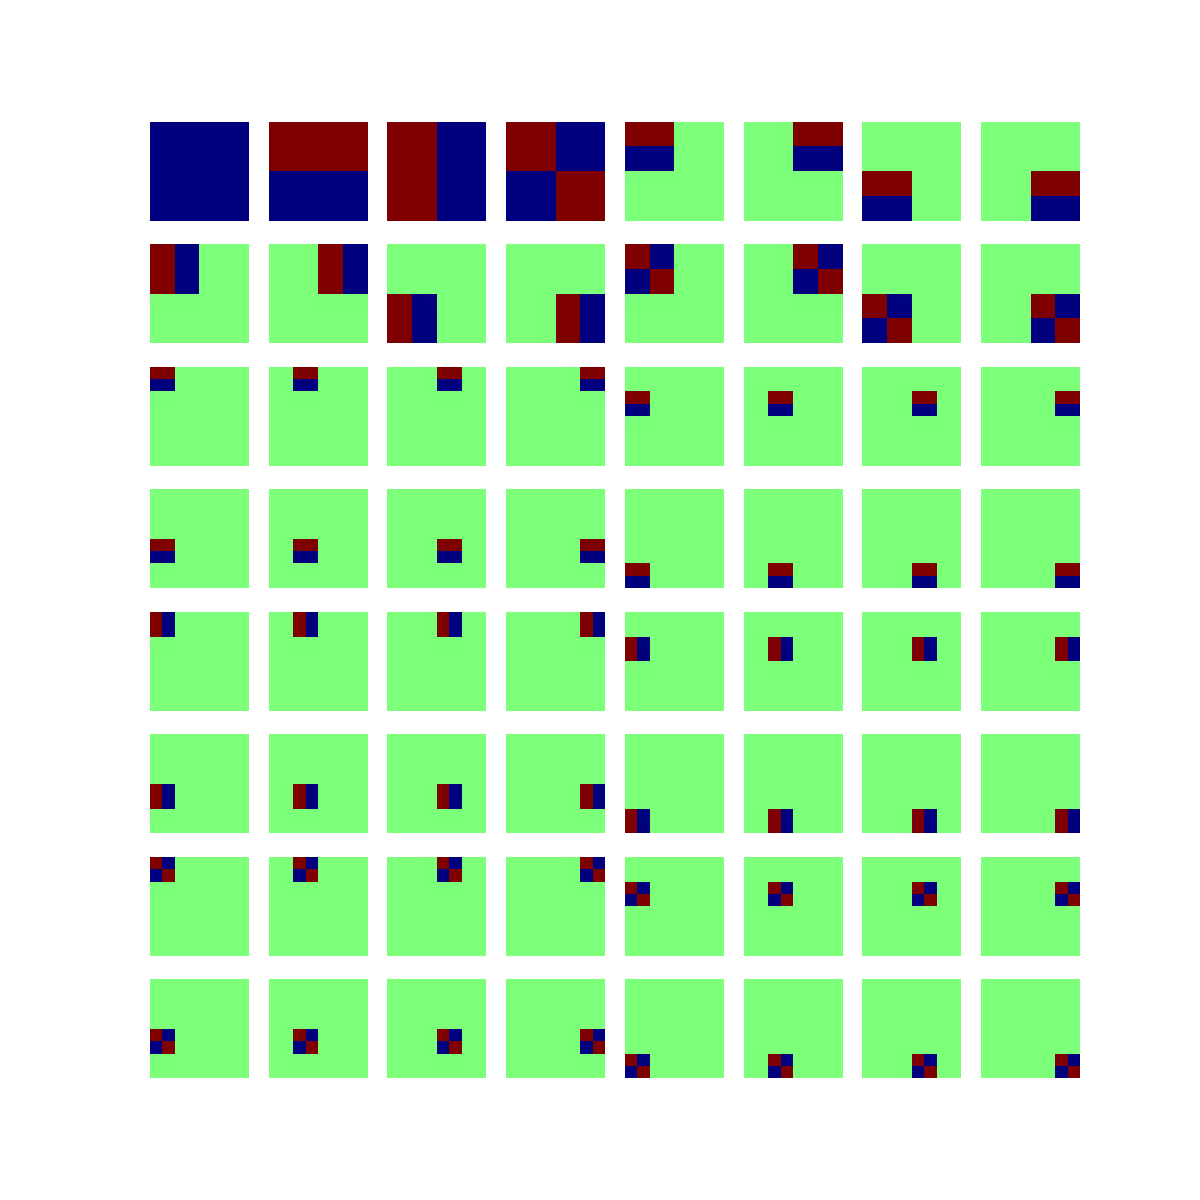
\includegraphics[width=.6\textwidth, trim={5em 4em 4em 4em}, clip]{Wavelets}\\
}{
	\vskip5em
    \centering
    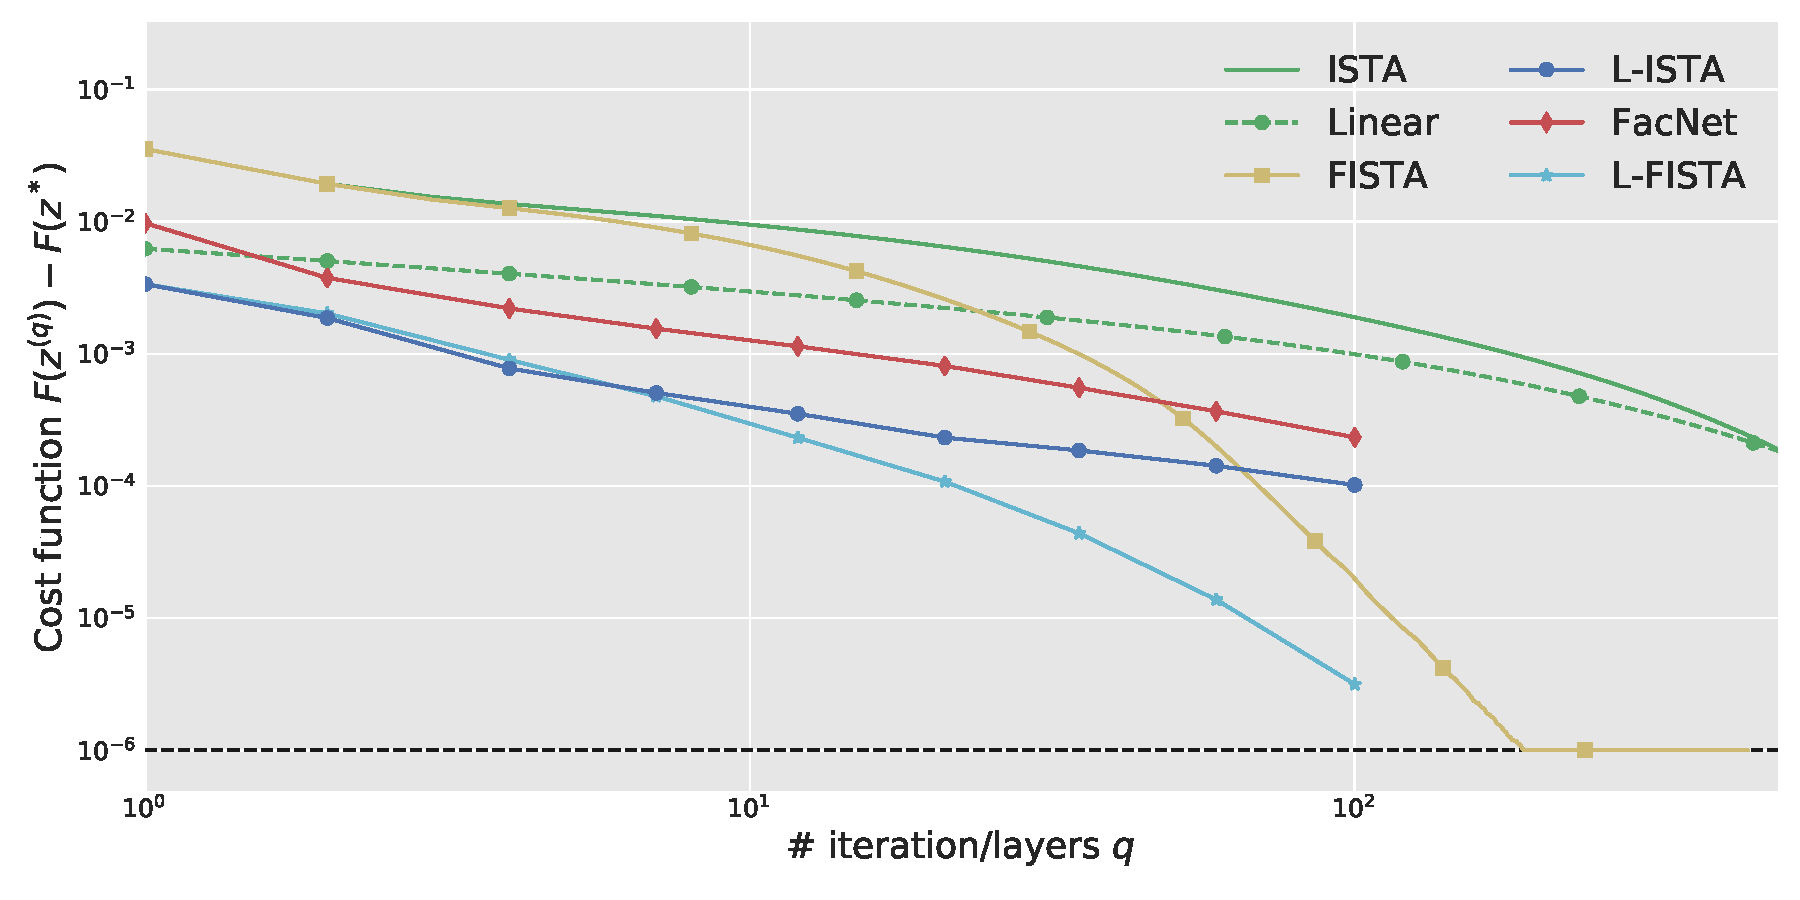
\includegraphics[width=\textwidth]{curve_images_seaborn}\\
     Evolution of the cost function $F(z^{(q)})-F(z^*)$ with the number of layers
     or the number of iteration $q$ for Pascal VOC 2008.
}
\end{frame}


\begin{frame}{MNIST}
\twocols{
	\btitle{MNIST}
	\vskip1em
	Dictionary $D$ with $K=100$ atoms learned on 10 000 MNIST samples (17x17) with dictionary learning.
	LISTA trained with MNIST training set and tested on MNIST test set.\\[1em]
}{
    \centering
    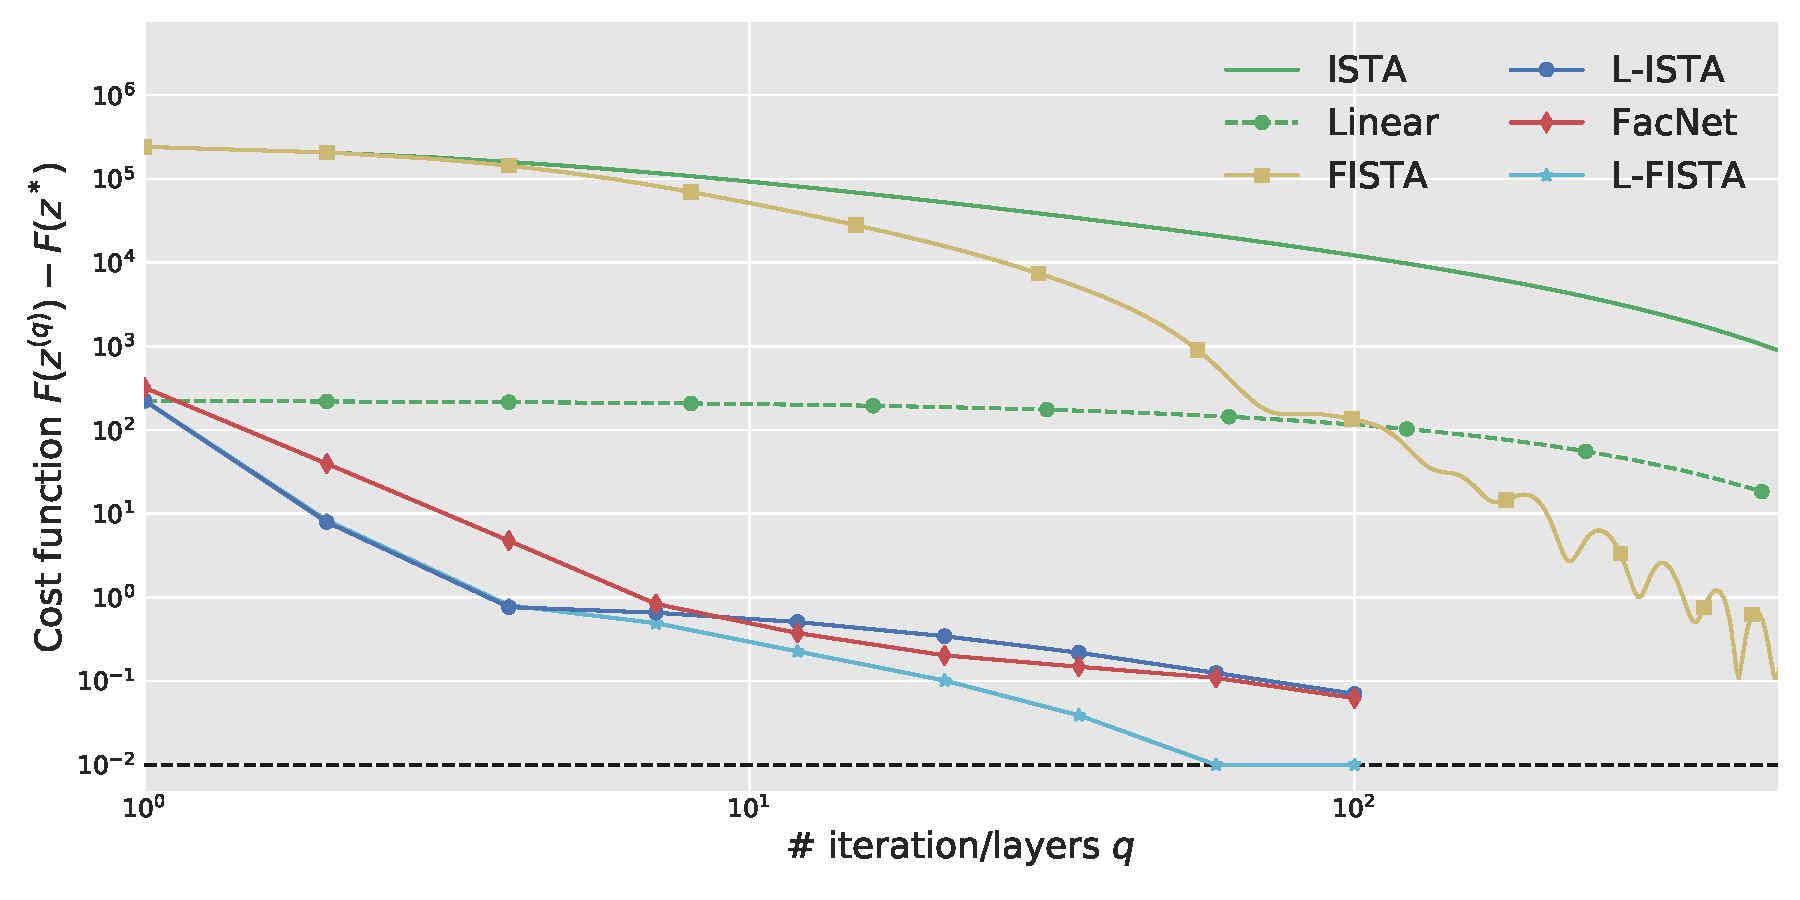
\includegraphics[width=\textwidth]{curve_mnist_seaborn}\\
     Evolution of the cost function $F(z^{(q)})-F(z^*)$ with the number
     of layers or the number of iteration $q$ for MNIST.
}{}
\end{frame}


%====================================================================
\subsection{DICOD}
%====================================================================

\begin{frame}{}

	\twocols{
	\btitle{Finishing the process in a linear grid?}
	Non trivial point: {\bf How to decide that the algorithm has converged?}\\[2em]
	
	\begin{itemize}\itemsep2em\itemindent1em
		\item Neighbors paused is not enough!
		\item Define a master 0 and send probes.\\
			\hskip3em Wait for $M$ probes return.
		\item Uses the notion of message queue and network flow.\\
			\hskip3emMaybe we can have better way?
	\end{itemize}
	}{}
	
	
\end{frame}

\begin{frame}
	\twocols{
		\centering
		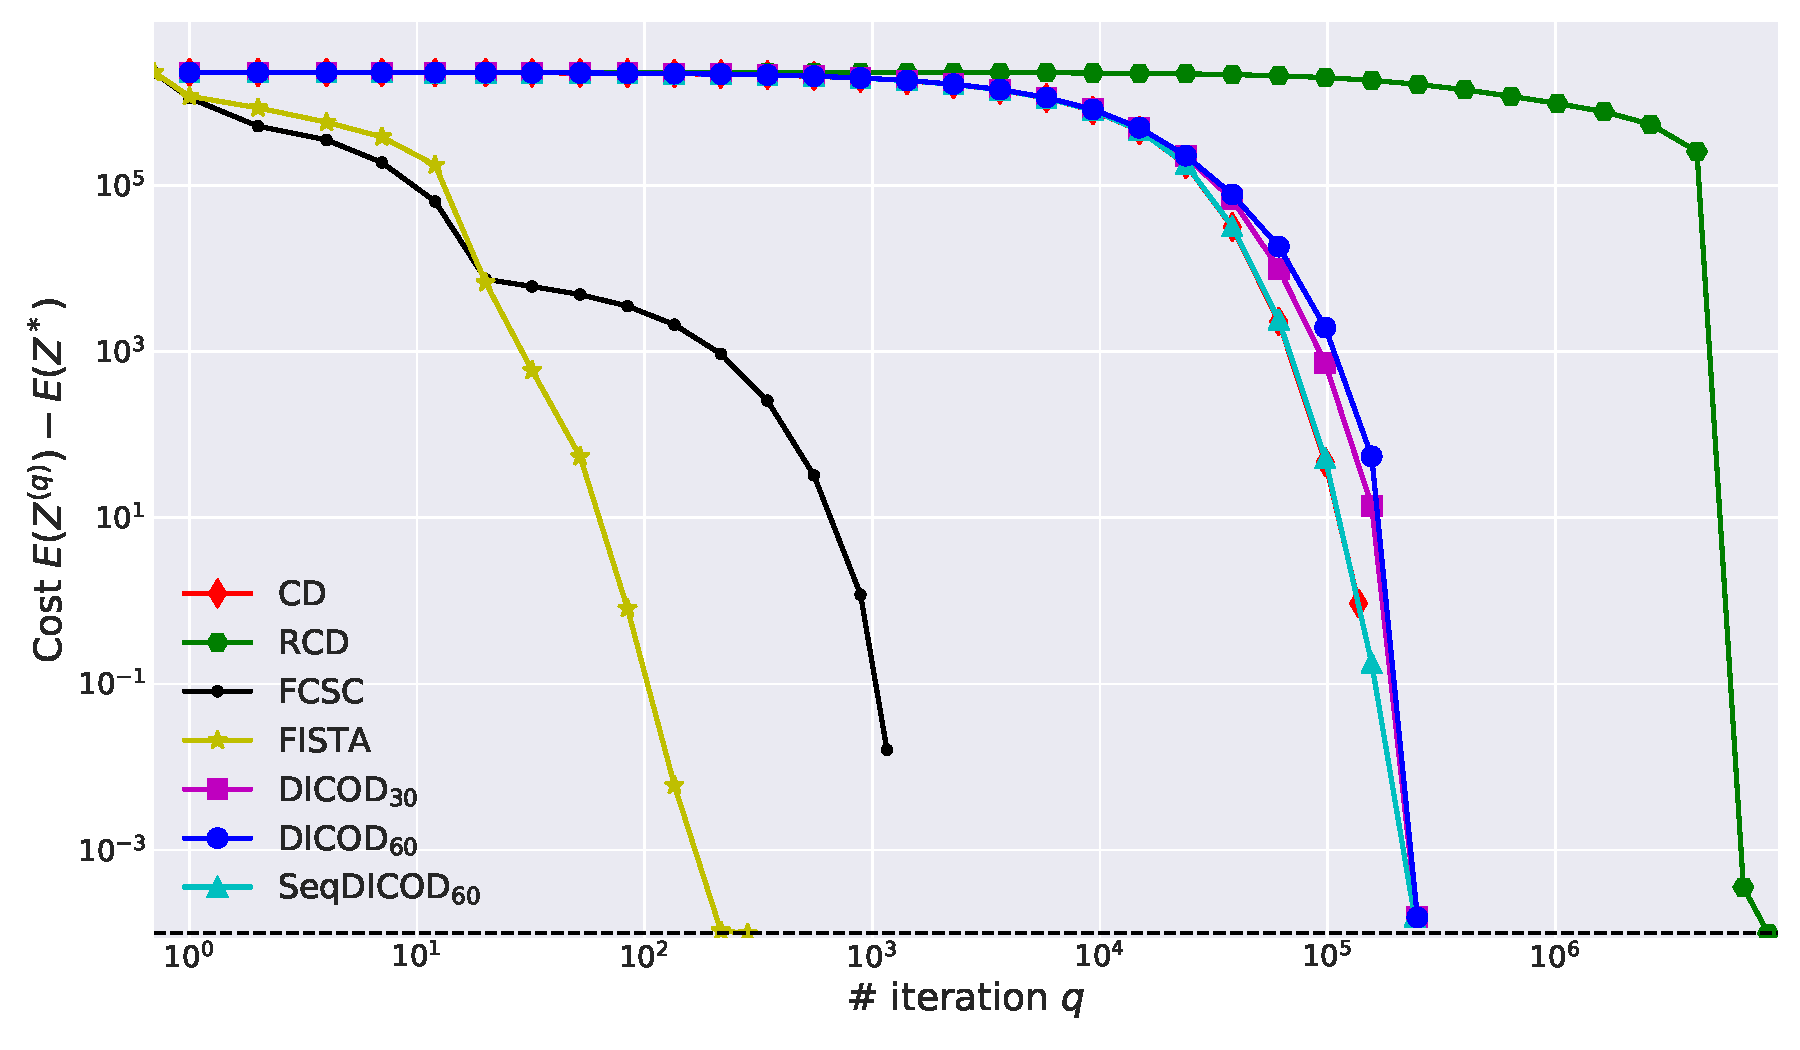
\includegraphics[width=\textwidth]{cost_seaborn_iter}\\
		\large Cost as a function of the iterations
	}{
		\centering
		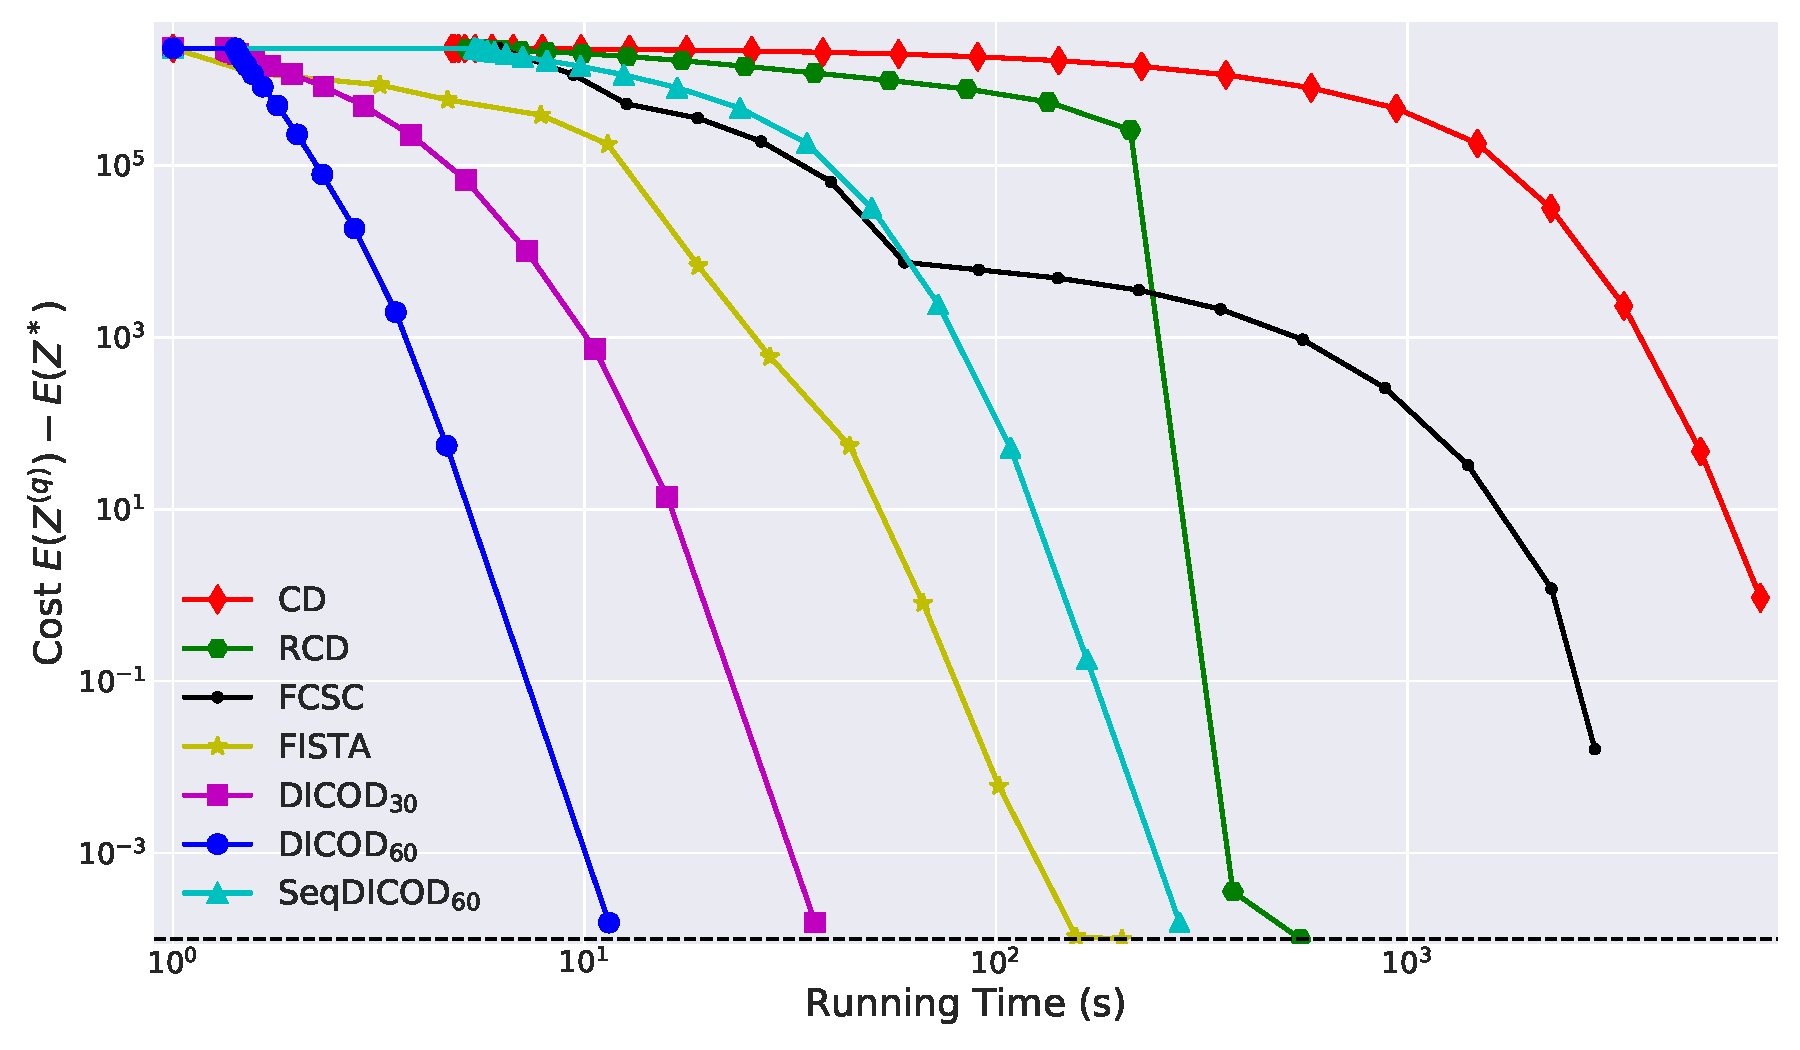
\includegraphics[width=\textwidth]{cost_seaborn_time}\\
		\large Cost as a function of the time
	}
\end{frame}



%====================================================================
\subsection{Singular Spectrum Analysis (SSA)}
%====================================================================

\begin{frame}{Singular Spectrum Analysis (SSA) \mycite{Vautard1989}}
	\twocols{
		\btitle{Sinuglar Spectrum Analysis}
		\vskip2em
		\begin{itemize}
			\item Choose a window size $K$ and extract sub series,
			\item Reconstruct a low rank estimate of all the $K$-length sub series,
			\item Decomposition of the series as a sum of "low rank" components.
		\end{itemize}
		}{
		{\usebeamercolor[bg]{itemize}.}\vskip2.5em
		\begin{itemize}\itemsep1em
		\item[$\rightarrow$] K-trajectory matrix $\pmb X^{(K)}$
		\item[$\rightarrow$] Singular Value decomposition
		$X^{(K)} = \sum_{k=1}^K \lambda_k U_kV_k^T$
		\item[$\rightarrow$] Average along anti-diagonals
	\end{itemize}
	}
	\vskip2em
	\bimplies{Extract components linked to trend and oscillations}
\end{frame}



\begin{frame}{Singular Spectrum Analysis}
\twocols{
	\vskip2em
	Linked to the convolutional least square
\begin{equation}\label{eq:sparse_code}
	Z^*, \pmb D^* = \arg\min_{Z, \pmb D} \frac{1}{2} \left\|X - \sum_{k=1}^K z_k*D_k\right\|_2^2,
\end{equation}
with constraints $\langle D_i, D_j \rangle = \delta_{i, j}$ 


\vskip1em
\begin{itemize}
	\item $\pmb D$ is the dictionary with $K = W$ patterns in $\mathbb R$ of length $W$
	\item $Z$ is an activation signal, or coding signal in $\mathbb R^K$ of length $L = T-W+1$
\end{itemize}
}{
	\vskip3em
	{\bf Issues}\\[1em]
	\begin{itemize}\itemsep1em\itemindent1em
	\item Same pattern present in different components,
	\item Representation is "dense", no localization,
	\item Different representation for each signal,
	\item A grouping step necessary to clean the extracted patterns.
	\end{itemize}
}
\end{frame}


\begin{frame}{Detrending with oculo}
	
\end{frame}



%====================================================================
\subsection{Post-training for Deep Learning}
%====================================================================


\begin{frame}{Post-training for Deep Learning}
\twocols{
	\btitle{Post-training}
	\vskip1em
	{\bf Paper with J. Audiffren: } arxiv:1611.04499\\[2em]

	Use the idea to split the representation learning and the task resolution:\\[1em]
	\begin{itemize}\itemindent1em\itemsep1.5em
		\item \underline{{\it Post-training} step:} only train the last layer,
		\item \underline{Easy problem:} this problem is often convex,
		\item \underline{Link with kernel:} close form solution for optimal last layer,
		\item \underline{Experiments:} consistent performance boost with multiple architecture.
	\end{itemize}
	}{
	\vskip3em
		{\bf Remarks}\\[1em]
	\begin{itemize}\itemsep1em\itemindent1em
	\item No gain if we are in a local minima,
	\item Should be use with early stopping.
	\end{itemize}
	}
	
\end{frame}



\end{document}
